\documentclass[final]{IEEEtran}
\usepackage[dvips]{epsfig}
\usepackage[english]{babel}
\usepackage{amsfonts}
\usepackage[dvips]{graphicx}
\usepackage{multirow}
\usepackage[dvips]{epsfig}
\usepackage{array}
\usepackage{amsmath}
\usepackage{url}
\usepackage{slashbox}
\usepackage{amssymb}
\usepackage{fancyhdr}

\def\BibTeX{{\rm B\kern-.05em{\sc i\kern-.025em b}\kern-.08em
    T\kern-.1667em\lower.7ex\hbox{E}\kern-.125emX}}

\newtheorem{theorem}{Theorem}
\setcounter{page}{1}

\begin{document}

\title{Evolving Scale-free Networks by Poisson Process: Modeling and Degree Distribution}

\author{Minyu Feng,  Hong Qu {\em Member, IEEE}, Zhang Yi {\em Senior Member,
IEEE} and Xiurui Xie
\thanks{This work was supported in part by the National Basic Research Program of China (973 Program) under Grant 2011CB302201 and in part by the National Science Foundation of China under Grants 61273308.
}
\thanks{Minyu Feng is with School
of Computer Science and Engineering, University of Electronic
Science and Technology of China, Chengdu 610054, P. R. China
(e-mail: fmy1987@sina.com). }
\thanks{Hong Qu is with School
of Computer Science and Engineering, University of Electronic
Science and Technology of China, Chengdu 610054, P. R. China
(e-mail: hongqu@uestc.edu.cn).}
\thanks{Zhang Yi is with College of Computer Science, Sichuan
University, Chengdu 610065, P. R. China (e-mail:
zhangyi@scu.edu.cn).}
\thanks{Xiurui Xie is with School
of Computer Science and Engineering, University of Electronic
Science and Technology of China, Chengdu 610054, P. R. China
(e-mail: xiexiurui@126.com). } }


\maketitle \thispagestyle{plain}\pagestyle{plain}



\begin{abstract}
Since the great mathematician Leonhard Euler initiated the study
of graph theory, the network has been one of the most significant
research subject in multidisciplinary. In recent years, the
proposition of the small-world and scale-free properties of
complex networks in statistical physics, made the network science
intriguing again for many researchers. One of the challenges for
the network science is to propose rational models for complex
networks. In this paper, in order to reveal the influence of the
vertex generating mechanism on complex network structure, we
propose three novel models based on the homogeneous Poisson,
nonhomogeneous Poisson and birth death process, respectively,
which can be regarded as typical scale-free networks utilizing to
simulate practical situation, such as social and financial
networks. The degree distribution and exponent are analyzed and
explained in mathematics by different approaches. In the
simulation, we display the modeling process, the degree
distribution of empirical data by statistical methods, and
reliability of proposed networks, results show our model follows
the feature of typical complex networks. Finally, some future
challenges for complex systems are discussed.
\end{abstract}

\begin{keywords}
Complex network modeling, Poisson process, Power-law distribution,
Degree distribution, Degree exponent, Reliability.
\end{keywords}
\maketitle\thispagestyle{plain}\pagestyle{plain}



\thispagestyle{fancy}
\renewcommand{\headrulewidth}{0cm}
\fancyfoot[C]{\footnotesize Copyright (c) 2014 IEEE. Personal use of this material is permitted. However, permission to\\
use this material for any other purposes must be obtained from the
IEEE by sending an email to pubs-permissions@ieee.org.}

\section{Introduction}
With rapid development of Internet, information technology has
become the focus of people's daily lives, and ushered the mankind
into the age of complex networks. Network science based on
information technology is now a significant issue and a useful
tool to man's activities of production. As we know, many practical
networks such as communication, traffic, social, and biological
networks are regarded as complex systems, having same properties
like small-world, scale-free, etc. However, practical networks are
difficult to study, the key issue of network science is to create
a virtual complex network model, which follows similar topology
characteristics of practical networks.

%The modern stage of network modeling started from the famous
%small-world experiment, which was made by Stanley Milgram
%\cite{Mil}. This experiment is also known as ``Six Degrees of
%Separation", regardless of its own limitations, it built a small
%group of network model and revealed the average distance between
%any two people is about $5.2$ and our world is very small, the
%short average path length is considered as an important property
%of practical networks.
In the late 20th century, two significant small-world models were
proposed by Watts and Strogtz, Newman and Watts \cite{Watts1},
\cite{Newman1}, respectively. They discovered that the practical
networks are neither regular networks nor random graphs and should
fall in between them, and realized them by randomly reconnecting
and adding edges. Significantly, their models achieved the goal of
low distance between any two vertices and first simulates the
small-world characteristic, the domination of $ER$ random graph
proposed by Erd\"{o}s and R\'{e}nyi in network science is finally
changed. However, both $ER$ random graph and $WS$ small-world
network have the same property that their degree distributions
follow a Poisson distribution, having a peak value in the average
degree that considered as exponential networks. However, the
recent researches reveal that, most practical networks follow
power-law distribution and are commonly called scale-free
networks. Barab\'{a}i and Albert are one of the first researchers
to study the issue, and they proposed the famous $BA$ scale-free
network model \cite{Barabasi}. They take the growth and
preferential attachment of practical networks into consideration,
and successfully construct a network with Power-law distribution.
Later, many methods such as the mean-field \cite{bah},
rate-equation \cite{kraa}, master-equation \cite{do} were proposed
to prove the Power-law character of scale-free networks. In
addition, there are many structure algorithms based on $BA$ model,
see \cite{doro}, \cite{jeong}, \cite{kra}, \cite{li}, \cite{cs},
and also other scale-free network models given realistic
consideration, see \cite{houu}, \cite{guang}, \cite{lian},
\cite{wen}, \cite{span}, \cite{hou}, \cite{sc}, \cite{ma}.

However, most of scale-free networks like $BA$ consider their
generation rate of vertices and number of connections as constant,
but in practical situation, all variable with time. If so, are
these networks still independent of time? In order to address this
issue, we propose a novel scale-free network based on the Poisson
process, which is an evolution of the $BA$ scale-free network. Our
model starts with a small group that highly gathered and connected
to each other, and in the processing of modeling, we employ the
homogeneous Poisson process to simulate the generation of
vertices, and Gaussian distribution to produce the connection
number. The dynamic method in physical and probabilistic approach
in mathematic are utilized to analyze the degree distribution and
its relationship with time. In addition, assuming that the
generation rate changes with time and existed individuals keep
dying, we extend this model to the nonhomogeneous Poisson and
birth and death situation, which are more close to practical
networks, and discuss their topologies. In the view of
application, these networks with variable generation rates can be
utilized to simulate the practical situation which is difficult to
obtain the data, and regarded as underlying models to solve issues
like search, synchronization, etc. In the simulation, we
demonstrate detailed construction process for three networks,
apply statistical approach to obtain the degree distribution and
exponent from empirical data, and measure the reliability of these
networks under deliberate and random attack.






This paper is organized as follows. A detailed presentation and
analysis of the homogeneous Poisson network is given in section
II. Introductions and analysis of nonhomogeneous Poisson and birth
and death network are presented in section III. Simulations are
carried out in section IV to demonstrate these networks follow
Power-laws and are scale-free. Finally, conclusions and outlooks
are drawn in Section VI.









\section{The Scale-free Network based on Homogeneous Poisson Process}

It is well known that the $BA$ scale-free network is one of the
first models to propose the growth characteristic, both $BA$
scale-free network and other similar networks simply consider that
one vertex or individual is connected to the existing network for
each unit time. However, for real networks, the generation of
vertices or individuals follows certain rules. For example, the
population network does not generate one individual each unit
time, differently, the growth rate changes all the time and is
decided by many factors such as wars, economies, etc.
Consequently, a common property of these networks is that the
generation possesses certain rate, which can be supposed as a
counting process.


Besides, a $BA$ scale-free network obtains permanent $m$ edges for
each vertex added in, but in real situation, connections of
different vertices are very mutable. For example,in the network of
the research reference, once a high quality paper such as
``Emergence of scaling in random networks" by Barab\'{a}si is
published, many related references will emerge in a short time.
Consequently, the number of connections is influenced by the
vertex's own fitness.

The network initialization issue is also undone by Barab\'{a}si.
Given realistic consideration, the individuals of an initial
network are often small group but highly gathered and connected to
each other. For instance, ARPANET, the precursor of Internet, had
only four vertices dispersed in four universities and connected to
each others. Consequently, the initialization phase of a complex
network is high clustering and has short distance.

Based on these these issues, we then show a novel model based on
the Poisson process that follows a Power-law distribution.




\subsection{Description of Proposed Model}

The main idea of our proposed model is to confirm the initial
network, growth mechanism, preferential connection and end time,
we summarize them as Initialization, Growth, Connection and
Termination and briefly introduce them below:

\textbf{Initialization}: Given $N$ vertices as a nearest-neighbor
coupled networks, in which each vertex connects to its $K/2$
neighbors on the left and the right; For any pair of vertices, an
extra connection is established by the probability of $p$.




\textbf{Growth}: Newly added vertices $i$ are coming by the rate
at $\lambda$; For each new vertex, $\eta_{i}$ edges are connected
to the existing vertices.



\textbf{Connection}: The probability of a newly added vertex
connected to an existing vertex is decided by $\Pi_{i}$.

\textbf{Termination}: As time reaches $T$, the algorithm
terminates and the network is output.




In Initialization, the size of an initial network is input as
$m_{0}$, and constructed as a $NW$ small-world network, the values
of $K$ and $p$ determine the degree of clustering, which can be
controlled to simulate different types of network. This step can
solve the unaddress issue of $BA$ network.

The Growth is the key section of our model, which is the main
improvement of $BA$ network, and the counting time starts from
this phase to simplify calculation. The generation of vertices
follows the rule of Poisson distribution, the detailed definition
is given below:

\newtheorem{myDef}{Definition}
\begin{myDef}\label{d1} The generation of new vertices ${N(t), t\gg0}$
is a Poisson process having rate $\lambda$, $\lambda>0$, and

\noindent$\diamond$ $N(0)=0$;

\noindent$\diamond$ The process has independent increments;

\noindent$\diamond$ The number of added vertices in any interval
of length $t$ is Poisson distributed with mean $\lambda t$, which
is, for all $s, t\geq0$,
\begin{equation}\footnotesize
P\{N(t+s)-N(s)=k\}=\frac{[\lambda(t-s)]^{k}}{k!}e^{-\lambda(t-s)},
k=0,1,\cdots
\end{equation}
\end{myDef}
\phantom{blahblah}



Then, different from $BA$ network, for each new vertex, the number
of connections is supposed to follow a Gaussian distribution as
its fitness function. The definition is expressed as:

\begin{myDef}\label{d2} For a newly added vertex
$i$, the number of connections $\eta_{i}$ is a Gaussian
distribution with parameters $\mu$ and $\sigma^{2}$, and the
density is given by
\begin{equation}\footnotesize
f(x)=\frac{1}{\sqrt{2\pi}\sigma}e^{-(x-\mu)^{2}/2\sigma^{2}}
0<x<+\infty
\end{equation}
where $x$ can only be an integer.
\end{myDef}


The fitness function denotes the adaptivity of a new vertex, the
higher value indicates the vertex is easier to fit in with the
network.

In Connection and Termination,  $\Pi_{k}$, the probability of a
connection to a vertex $i$, is denoted as:
\begin{equation}\label{e1}\footnotesize
\Pi(k_{i})=\frac{k_{i}}{\sum \limits_{j}k_{j}}
\end{equation}
where $k_{i}$ is the degree of a vertex $i$, $i$ denotes all
existed vertices. We utilize the roulette to select the vertex to
be connected. Repeated connection is avoided. $T$ is the time of
termination, which can be controlled.


\subsection{Demonstration of the Network Evolution}

In this subsection, we present an example of the Poisson based
scale-free model and explain its evolution in details. In order to
describe with clarity, the parameters are listed in Tab. \ref{t1}.

\begin{table}[htbp]\tiny
\begin{center}
\caption{\label{t1} The parameters for the demonstration.}
\begin{tabular}{|c|c|c|c|c|c|c|c|}
\hline Parameter & $N$  & $K$   & $p$ & $\lambda$ & $\eta$ & $T$\\
\hline
   Value  & 5  & 2   & 0.1  & 1 &1, 2 & 10\\
\hline
 \end{tabular}
\end{center}
\begin{scriptsize}
where $N$ denotes the number of the initial network, $K$ denotes
the number of connections to neighbors, $p$ is the probability of
a new connection, $\lambda$ denotes the rate of the generation,
$\eta$ is the number of connections, and $T$ denotes the terminal
time of generated vertex.
\end{scriptsize}
\end{table}


\begin{figure}[!htp]
\centering
 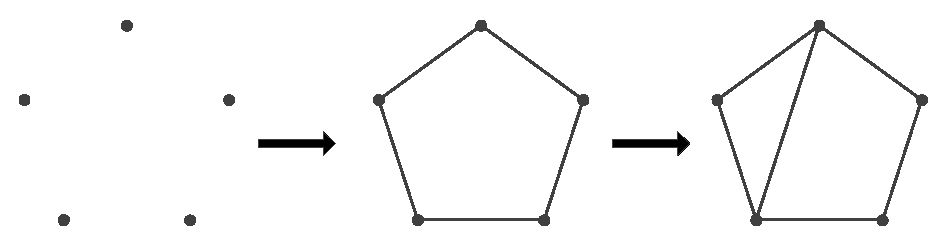
\epsfig{file=1.eps, scale=0.35}
\caption{\label{f1}Initialization: 5 vertices are connected as a
nearest-neighbor coupled network, with each vertex connecting to
its neighbor on the left and the right, and adding edges by the
probability 0.1.}
\end{figure}
\begin{figure}[!htp]
\centering
 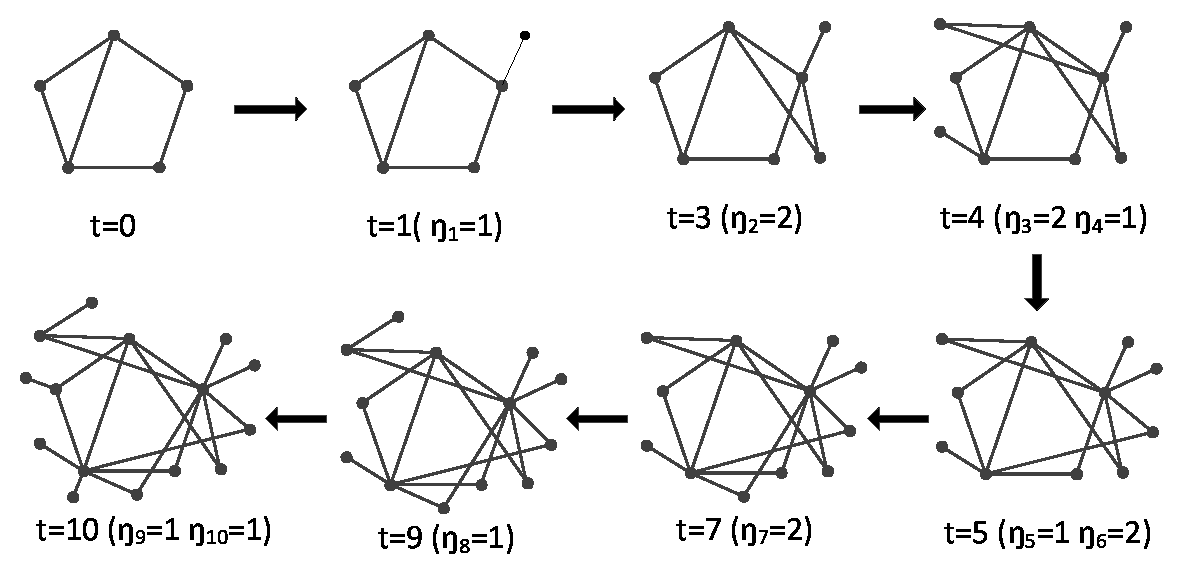
\epsfig{file=2.eps, scale=0.38}
\caption{\label{f2}Homogeneous Poisson network evolution: new
vertices are generated by the mean rate 1 and connects to one or
two existed vertex, the generation is terminated at time $10$.}
\end{figure}

The detailed construction is illustrated in Fig. \ref{f1} and
\ref{f2}. Fig. \ref{f1} simulates the process of building an
initial network, which is a simple small-world network and only
one extra edge is connected as a shortcut. Fig. \ref{f2} contains
the network evolution of the growth, connection and termination.
From this figure, we can see that the mean rate
$\lambda=(1+1+2+2+1+1+2)/10=1$. According to Def. \ref{d1}, the
generation follows a Poisson process with mean rate $1$. And once
a new vertex arrives, the values of connections to exist vertices
are decided by a Gaussian distribution with the value
$\eta_{i}\in\{1,2\}$. Obviously, the poor vertices with the degree
below $4$ are in the majority ($80\%$) in this network, and the
rich vertices with the degree upon $4$ are in minority ($20\%$),
which is commonly referred to as ``the Matthew effect" or ``the
rich-get-richer phenomenon", and also the property of a power-law
distribution.

%When time
%reaches $10$, the evolution is terminated. %It is mentionable that,
%%in this figure, in order to express conveniently, the shortest
%%unit time is set as $1$, which means if two new vertices arrives
%%at time $1.65$ (t=1.65) and $1.8$ (t=1.8), we consider that they
%%both generates at time $2$ (t=2).
%
%
%The degree distribution of this figure is provided as $\{1, 3, 5,
%8, 1, 1, 2, 2, 2, 2, 7, 1, 1, 1, 3\}$,
%\begin{table}[htbp]\tiny
%\begin{center}
%\caption{\label{t2} The degree of each vertex in Fig. \ref{f2}
%($t=10$).}
%\begin{tabular}{|c|c|c|c|c|c|c|}
%\hline Degree & 1 & 2   &3 & 5 & 7 & 8\\
%\hline
%   Number  & 6  & 4   & 2  & 1 &1 &1\\
%\hline
% \end{tabular}
%\end{center}
%\end{table}
%\begin{figure}[!htp]
%\centering
% 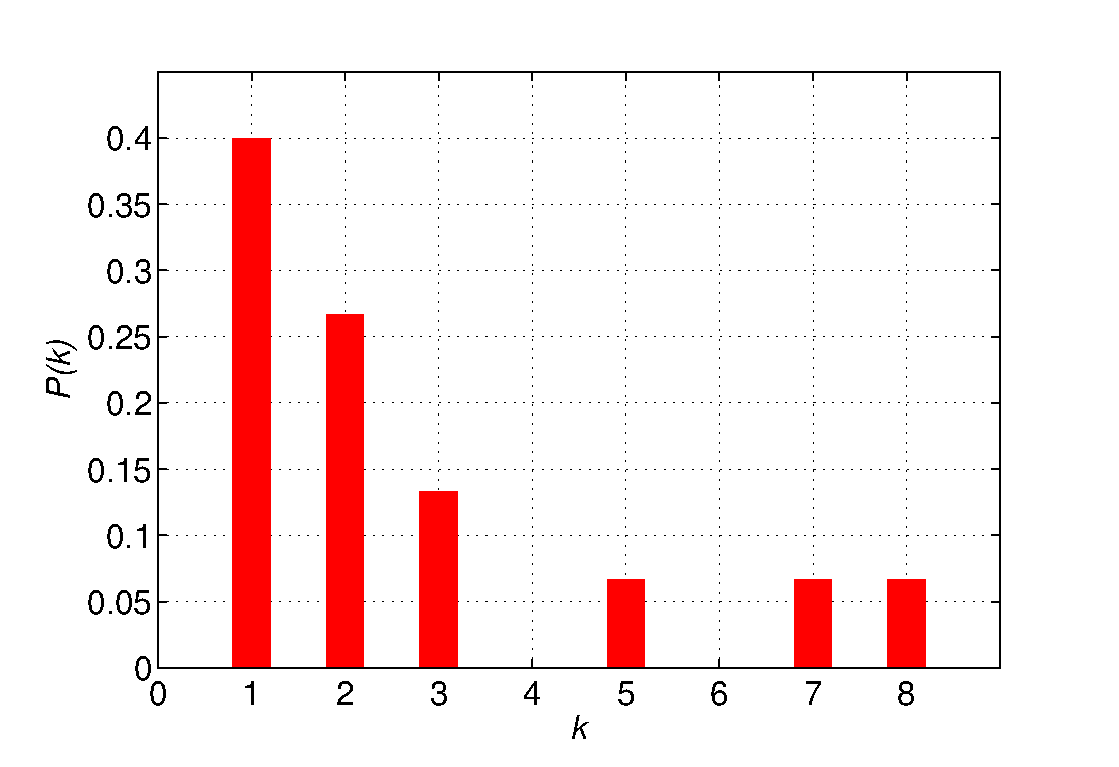
\epsfig{file=3.eps, width=5.5cm, height=4cm, angle=0}
%\caption{\label{f3}The discrete degree distribution for Fig.
%\ref{f2} ($t=10$): $k$ is the degree, $P(k)$ is the probability
%that the degree is just $k$.}
%\end{figure}


%The clustering coefficient is expressed as:
%\begin{equation}
%C_{i}=\frac{2E_{i}}{k_{i}(k_{i}-1)}
%\end{equation}
%where $k_{i}$ denotes the number of neighbors of the vertex $i$,
%$E_{i}$ is the number of connections of $k_{i}$. The clustering
%coefficient of each vertex is $\{1/3, 1/5, 1/14, 0, 1, 0, 0, 1/21,
%0\}$ (The vertices with $1$ degree are abandoned). And the average
%clustering coefficient of this figure is
%\begin{equation}
%\overline{C}=\frac{\frac{1}{3}+\frac{1}{5}+\frac{1}{14}+0+1+0+0+\frac{1}{21}+0}{9}\approx0.1836\nonumber
%\end{equation}

\subsection{Fitting Proposed Model in A Network of Coauthorships}
One of the potential application of the homogeneous Poisson
network is to simulate the practical networks since they have many
common characters such as the growth following the Poisson
process, the connection following the Gauss distribution and the
preferential attachment. In this subsection, we give a simple
example to fit a homogeneous Poisson network in a network of
coauthorships.

The database is a network of coauthorships between scientists,
scientists in this case who are themselves publishing on the topic
of networks which was studied by Newman \cite{data}.

To fit the real-world network, the parameter of growth and
connection is required, and our object is to extract these data
from the coauthorship network. As described in Ref. \cite{data},
the network started from two articles by Newman and Boccaletti,
which indicate the initial network has only two connected
vertices. The articles are published from $2003$ to $2006$ and a
total of $1589$ scientists are included in the network, then we
suppose the growth rate $\lambda$$=$$44.14$ per month and
termination time $T$$=$$36$. From observation, we find the
connection of each vertex is between $1$ and $5$, which can be
considered as a Gauss distribution with $\mu$$=$$3$ and
$\sigma$$=$$2$. With these arguments from the coauthorship
network, we can build a homogeneous Poisson network by our method
as described before.

\begin{figure}[!htp]
\centering
 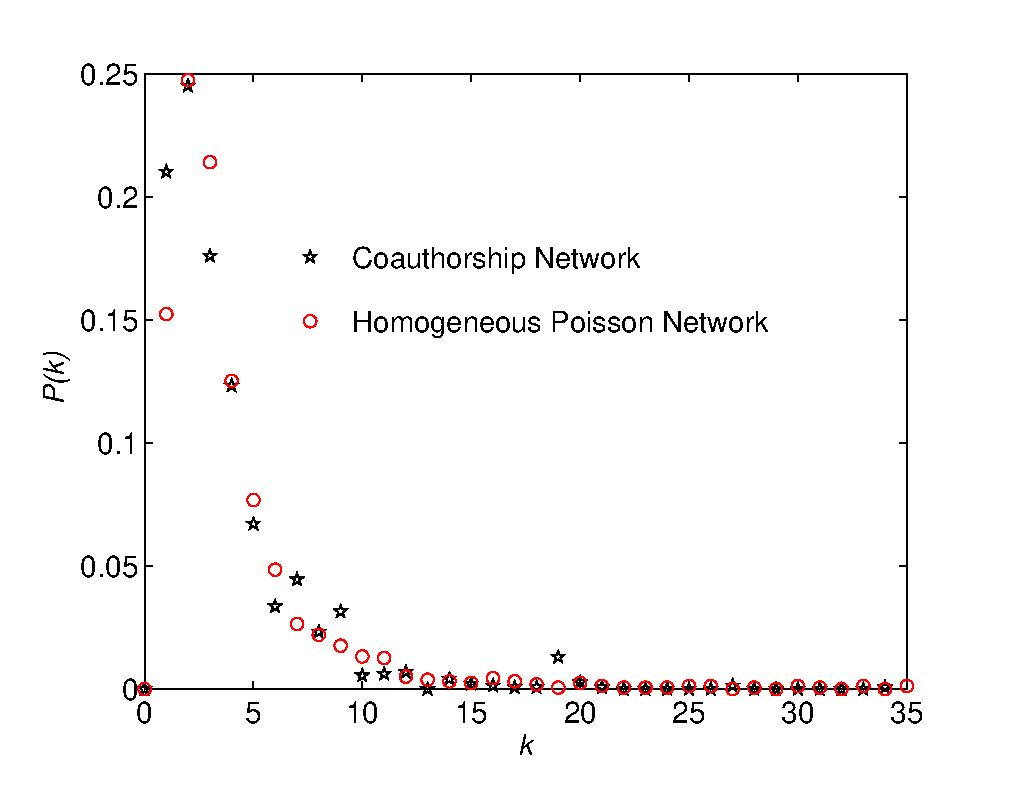
\epsfig{file=xxx.eps, scale=0.4}
\caption{\label{fx} The degree distribution of the coauthorship
network and homogeneous Poisson network, the values of P(k) are
(0, 0.1523, 0.2473, 0.2140, 0.1252, 0.0768, 0.0485, 0.0264,
0.0220, 0.0176, 0.0132, 0.0126, 0.0050, 0.0038, 0.0031, 0.0025,
0.0044, 0.0031, 0.0019, 0.0006, 0.0025, 0.0013, 0.0006, 0.0006,
0.0006, 0.0013, 0.0013, 0, 0.0006, 0, 0.0013, 0.0006, 0, 0.0013,
0)
 and (0, 0.1523, 0.2473, 0.2140, 0.1252,
0.0768, 0.0485, 0.0264, 0.0220, 0.0176, 0.0132, 0.0126, 0.0050,
0.0038, 0.0031, 0.0025, 0.0044, 0.0031, 0.0019, 0.0006, 0.0025,
0.0013, 0.0006, 0.0006, 0.0006, 0.0013, 0.0013, 0, 0.0006, 0,
0.0013, 0.0006, 0, 0.0013, 0).}
\end{figure}

After the theoretical model is obtained, we mainly compare its
degree distribution with the practical coauthorship network's, the
result is shown in Fig. \ref{fx}. Then, we employ the correlation
coefficient of their degree distributions to calculate the fitness
of these two networks, that is
\begin{equation}\footnotesize
\rho_{d_{c}d_{h}}=\frac{cov(d_{c},d_{h})}{\sqrt{Var(d_{c})}\sqrt{Var(d_{h})}}=0.9772
\end{equation}
where $cov$ denotes the covariance, $Var$ denotes the variance,
$d_{c}$ is the vector of the frequency from degree $1$ to $35$ of
the coauthorship network, and $d_{h}$ is the vector of the
frequency from degree $1$ to $35$ of the homogeneous network,
which are listed in the illustration of Fig. \ref{fx}. The value
of $\rho_{d_{c}d_{h}}$ indicates the fitness of vector $d_{c}$ and
$d_{h}$.

The result of correlation coefficient reveal that our proposed
model has a good performance on fitting in the coauthorship
network in the topology like the degree distribution. However,
it's complex to decide whether a academic model is perfectly
fitted in a practical network, many factors should be taken into
consideration and further study is required.

\subsection{Theoretical Analysis of the Proposed Model}
As we know, the scale-free is one of the most important topology
for complex networks. In this section, we focus on proving the
proposed model is a scale-free network, which is, given a fixed
$\lambda$, the degree exponent of this network is unrelated to the
construction time.

We utilize two approaches to accomplish the proof. Before the
proof carries out, some important definitions are provided first.

\begin{myDef}\label{d3}
At time $t$, the probability that the degree of a random vertex in
the network is exactly $k$, denoted by $P_{k}(t)$, is said to be a
\textbf{transient degree distribution}.
\end{myDef}

\begin{myDef}\label{d4}
Assuming that $P_{k}(i, t)$ denotes the probability that, at time
$t$, the degree of vertex $i$ is exactly $k$, and the initial
network is ignored, then the average probability
\begin{equation}\footnotesize
P_{k}(t)=\frac{\sum \limits_{i}P_{k}(i, t)}{t}
\end{equation}
is called the \textbf{average degree distribution} for the network
at time $t$.
\end{myDef}

\begin{myDef}\label{d5}
If $\lim \limits_{t\rightarrow\infty}P_{k}(t)$ exists and is equal
to $P(k)$, then $P(k)$ is said to be the \textbf{steady state
degree distribution} of this network.
\end{myDef}

%\begin{myDef}\label{d6}
%$\delta(x)$ is called \textbf{Dirac $\delta$-function} and
%\begin{equation}\footnotesize
%    \delta(x-k)=\left\{
%   \begin{aligned}
% &+\infty, \hspace{0.5cm}x=k\\
%&0, \hspace{1.1cm}x\neq k\\
%   \end{aligned}
%   \right.
%\end{equation}
%its integral follows
%\begin{equation}\footnotesize
%\int_{-\infty}^{+\infty}\delta(x-k)dx=1
%\end{equation}
%\end{myDef}
\phantom{blahblah}

Def. \ref{d3} and \ref{d4} provide two different forms of the
degree distribution at time $t$, and Def. \ref{d5} is the target
of our proof. As t$\rightarrow$$\infty$, the small initial network
has little effect on the degree distribution, therefore, in the
proof below, the initial network is ignored, which is, $t$$=$$0$,
the number of vertex is $0$. All the lemma and theorems proven
below are based on the homogeneous Poisson model.

\newtheorem{lemma}{Lemma}
\begin{lemma}\label{l1}
Given a fixed arrival rate $\lambda$ and an expected connection
$\mu$, the expectation of total degree at time $t$ is $2\lambda
\mu t$.
\end{lemma}
\begin{proof}
Suppose that $N(t)$ denotes the number of vertices at time $t$,
$\eta$ denotes the number of connections, then $E[N(t)\eta]$
denotes the total number of edges at time $t$, and by definition,
$E[N(t)]$$=$$\lambda t$ and $E[\eta]$$=$$\mu$.

The number of vertices is independent of connections, therefore,
the covariance is $0$, that is
\begin{equation}\footnotesize
cov(N(t),\eta)=E[N(t)\eta]-E[N(t)]E[\eta]=0
\end{equation}
scilicet,
\begin{equation}\footnotesize
E[N(t)\eta_{i}]=E[N(t)]E[\eta_{i}]=\lambda\mu t
\end{equation}

The total degree is two times of the total edges, and according to
the properties of expectation,
\begin{equation}\footnotesize
E=E[2N(t)]E[\eta_{i}]=2\lambda\mu t
\end{equation}

The result follows.

\end{proof}

\begin{theorem}\label{t1}
Given a fixed arrival rate $\lambda$, the degree exponent of the
proposed network is independent of time.
\end{theorem}

The first proof derives from the dynamics method which is widely
used by physicists:

\begin{proof}
Suppose that $k_{i}(t)$ is the degree of vertex $i$ at time $t$,
according to Lemma. \ref{l1}, at time $t$, the total degree is
\begin{equation}\footnotesize
\sum\limits_{j}k_{j}\approx2\lambda\mu t
\end{equation}

For each new vertex with $\eta$ connections, the probability that
an edge connects to the existed vertex $i$ is approximated as
\begin{equation}\label{e11}\footnotesize
P=\Big(^{\eta}_{1}\Big )
[\Pi(k_{i})][1-\Pi(k_{i})]^{\eta-1}\approx\eta\Pi(k_{i})=\frac{\eta
k_{i}}{2\lambda\mu t}
\end{equation}
where $\Pi(k_{i})$ is defined by Eq. \ref{e1}.

As we know, $\lambda$ new vertices generate per unit time, and the
degree growth rate of vertex $i$ is $\lambda P$. Then, $k_{i}(t)$
can be regarded as a dynamic equation based on the continuum
theory, and follows
\begin{equation}\footnotesize
  \left\{
   \begin{aligned}
   &\frac{\partial k_{i}(t)}{\partial t} \approx \lambda P =\frac{\eta
k_{i}(t)}{2\mu t}\\
&k_{i}(\frac{i}{\lambda})=\eta\\
   \end{aligned}
   \right.
  \end{equation}
the solution is
\begin{equation}\label{e2}\footnotesize
k_{i}(t)=\eta(\frac{\lambda t}{i})^{\frac{\eta}{2\mu}}
\end{equation}
where $\frac{\eta}{2\mu}$ is the kinetic index whose expectation
is $\frac{1}{2}$.

Assuming that vertex $i$ is randomly selected from $\lambda t$
vertices and follows a homogeneous distribution, that is,
$p(i)$$=$$\frac{1}{\lambda t}$, according to Eq. \ref{e2}, the
transient degree distribution is
\begin{equation}\footnotesize
P\{k_{i}(t)<k\}=P\{i>\lambda
t(\frac{k}{\eta})^{-\frac{2\mu}{\eta}}\}=1-\frac{\lambda
t(\frac{k}{\eta})^{-\frac{2\mu}{\eta}}}{\lambda t}
\end{equation}
the partial derivatives of $k$ is
\begin{equation}\footnotesize
P_{k}(t)=\frac{\partial P\{k_{i}(t)<k\}}{\partial
k}=2\mu\eta^{\frac{2\mu}{\eta}-1}k^{-(\frac{2\mu}{\eta}+1)}
\end{equation}
then, the steady state distribution is
\begin{equation}\label{eq16}\footnotesize
P(k)=\lim\limits_{t\rightarrow\infty}P_{k}(t)=2\mu\eta^{\frac{2\mu}{\eta}-1}k^{-\gamma}
\end{equation}
where $\gamma$$=$$\frac{2\mu}{\eta}+1$ and is independent of time
$t$.

The result follows.
\end{proof}

The alternative proof is based on the probabilistic approach and
commonly used by mathematicians:

\begin{proof}
Suppose that $k_{i}(t)$, the degree of vertex $i$ at time $t$,
denotes a stochastic variable, and $P_{k}(i,t)$ denotes the
probability that the degree of vertex $i$ is $k$ at time $t$.
Suppose that in unit time, $\lambda$ new vertices are generated,
each with $\eta$ connections, then the probability that an edge
connects to the existed vertex $i$ is approximated

\begin{equation}\footnotesize
P'=\Big(^{\lambda}_{1}\Big ) P(1-P)^{\lambda-1}\approx \lambda P
\approx \frac{\eta k}{2\mu t}
\end{equation}
where $P$ follows Eq. \ref{e11}.

Hence, the the connectivity distribution of a vertex obeys the
following master equation:
\begin{equation}\footnotesize
P_{k}(i, t+1)\approx \frac{\eta (k-1)}{2\mu
t}P_{k-1}(i,t)+(1-\frac{\eta k}{2\mu t})P_{k}(i,t)
\end{equation}
that is,
\begin{equation}\label{ex}\footnotesize
2\mu t[P_{k}(i, t+1)-P_{k-1}(i,t)]=-\eta [kP_{k}(i,
t)-(k-1)P_{k-1}(i,t)]
\end{equation}
Eq. \ref{ex} is a difference equation, and based on the continuum
theory, can be regarded as a partial differential equation, which
is:
\begin{equation}\label{e3}\footnotesize
2\mu t\frac{\partial P_{k}(i, t)}{\partial t}=-\eta\frac{\partial
[kP_{k}(i, t)]}{\partial k}
\end{equation}

Assuming that the expected degree function of vertex $i$ is:
\begin{equation}\footnotesize
\overline{k}(i,t)=\sum\limits_{k=0}^{\infty}kP_{k}(i,t)\approx\int_{0}^{\infty}kP_{k}(i,t)dk
\end{equation}

Then, by integral definition of $\overline{k}(i,t)$ and the
integration by parts of definite integral,
\begin{equation}\label{e4}\footnotesize
\begin{aligned}
&\hspace{0cm} \overline{k}(i,t)=-\{0-\int_{0}^{\infty}kP_{k}(i,t)dk\}\\
&\hspace{0.75cm}
=-\{[k^{2}P_{k}(i,t)]_{0}^{\infty}-\int_{0}^{\infty}kP_{k}(i,t)dk\}\\
&\hspace{0.75cm}
=-\int_{0}^{\infty}kd[kP_{k}(i,t)]=-\int_{0}^{\infty}kdk\frac{\partial
[kP_{k}(i, t)]}{\partial k}
\end{aligned}
\end{equation}


Eq. \ref{e3} can be converted into
\begin{equation}\footnotesize
2\mu t \int_{0}^{\infty}kdk\frac{\partial P_{k}(i, t)}{\partial
t}=-\eta\int_{0}^{\infty}kdk\frac{\partial [kP_{k}(i,
t)]}{\partial k}
\end{equation}
considering Eq. \ref{e4}, that is
\begin{equation}\footnotesize
\frac{\partial \overline{k}(i,t)}{\partial
t}=\frac{\eta\overline{k}(i,t)}{2\mu t}
\end{equation}

Thereupon, the partial differential equation turns into
\begin{equation}\footnotesize
  \left\{
   \begin{aligned}
   &\frac{\partial \overline{k}(i,t)}{\partial
t}=\frac{\eta\overline{k}(i,t)}{2\mu t}\\
&\overline k(i,\frac{i}{\lambda})=\mu\\
   \end{aligned}
   \right.
  \end{equation}
its general solution is $\overline{k}=t^{\frac{\eta}{2\mu}}C$, and
with the substitution of the condition, the result is
\begin{equation}\footnotesize
\overline{k}=\mu(\frac{\lambda t}{i})^{\frac{\eta}{2\mu}}
\end{equation}
and we can obtain
\begin{equation}\label{eq26}\footnotesize
i=\lambda t(\frac{\mu}{k})^{\frac{2\mu}{\eta}}
\end{equation}

Discrete distributions are described as continuous Dirac
$\delta$-function, then according to Def. \ref{d4}, our degree
distribution can be denoted as
\begin{equation}\label{eq27}\footnotesize
\begin{aligned}
&\hspace{0cm}P_{k}(t)=\frac{1}{t}\sum \limits_{i}^{\lambda t}
P_{k}(i,t)=\frac{1}{t}\int_{0}^{\lambda t}
P_{k}(i,t)\\
&\hspace{0.7cm}=\frac{1}{t}\int_{0}^{\lambda
t}\delta(k-\overline{k}_{i}(t))di=-\frac{1}{t}\int_{0}^{\lambda
t}\delta(\overline{k}_{i}(t)-k)di
\end{aligned}
\end{equation}
obviously,
\begin{equation}\footnotesize
d\overline{k}_{i}(t)=-\frac{\partial \overline{k}_{i}(t)}{\partial
i}di
\end{equation}
insert it in Eq. \ref{eq27}, we obtain that
\begin{equation}\label{eq28}\footnotesize
\begin{aligned}
&\hspace{0cm}P_{k}(t)=-\frac{1}{t}(1/\frac{\partial
\overline{k}_{i}(t)}{\partial
i})\int_{0}^{\lambda t}\delta(\overline{k}_{i}(t)-k)d\overline{k}_{i}(t)\\
&\hspace{0.7cm}=-\frac{1}{t}(1/\frac{\partial
\overline{k}_{i}(t)}{\partial i})=\frac{2i}{\eta
t}(\frac{i}{\lambda t})^{\frac{\eta}{2\mu}}
\end{aligned}
\end{equation}

According to Def. \ref{d5}, Eq. \ref{eq26} and \ref{eq28}, the
steady state degree distribution is
\begin{equation}\label{eq30}\footnotesize
\begin{aligned}
&\hspace{0cm}P(k)=\lim\limits_{t\rightarrow\infty}P_{k}(t)=\lim\limits_{t\rightarrow\infty}(\frac{2
i}{\eta t}(\frac{i}{\lambda t})^{\frac{\eta}{2
\mu}})|_{i=\lambda t(\frac{\mu}{k})^{\frac{2\mu}{\eta}}}\\
&\hspace{0.6cm}=2\lambda\mu^{1+\frac{2\lambda\mu}{\eta}}\eta^{-1}k^{-\gamma}
\end{aligned}
\end{equation}
where $\gamma$$=$$\frac{2\mu}{\eta}+1$ and is independent of time
$t$.

The result follows.
\end{proof}

Due to the different proof approaches, Eq. \ref{eq16} and
\ref{eq30} display a little difference, but if we seek their
expectations, the result is
\begin{equation}\footnotesize
P(k)=2\lambda\mu^{2\lambda}k^{-\overline{\gamma}}
\end{equation}
where $\overline{\gamma}$$=$$3$.

Obviously, when $\lambda$ is fixed, the conclusion is that our
proposed model is independent of time and follows the conception
of the scale-free network.

However, this is just a fundamental and ideal model, many
variables should be taken into consideration, such as variable
rates, mortality rate of vertices. Therefore, based on the
homogeneous Poisson scale-free model, we propose two extension
models and discuss whether they are still free of time.

\section{Various Extensions of the Poisson Scale-free Model}
As we discuss above, the generation rate of many complex networks
changes all the time. In different periods, the rate is also
distinct, for example, the population network during war years is
quite different than in peace time. This phenomenon of complex
networks is a typical nonhomogeneous process. Additionally, most
of complex models are simply a pure birth process which means the
vertices are always increasing, but in fact, individuals not only
generates but also vanishes in any kind of networks, for
instances, the species extinction in food chain networks, the
bankruptcy of a company in banking network, all of these networks
present the birth and death characteristics.

Based on these two viewpoints, in this section, we proposed two
various extension model- nonhomogeneous Poisson network model,
birth and death network model.

\subsection{Nonhomogeneous Poisson Network}
The construction algorithm of this model is close to Section II.
A: Initialization, Growth, Connection and Termination, the only
difference is in Growth:

%\textbf{Initialization}: Given $N$ vertices as a nearest-neighbor
%coupled networks, in which each vertex connects to its $K/2$
%neighbors on the left and the right; For any pair of vertices, an
%extra connection is established by the probability of $p$.




\textbf{Growth}: Newly added vertices $i$ are coming by the rate
at $\lambda(t)$; For each new vertex, $\eta_{i}$ edges are
connected to the existing vertices.



%\textbf{Connection}: The probability of a new added vertex
%connected to an existing vertex is decided by $\Pi_{i}$.
%
%\textbf{Termination}: As time reaches $T$, the algorithm
%terminates and the network is output.

The generation rate relates to the time $t$, which is often
denoted as $\lambda (t)$, and called a nonhomogeneous Poisson
process, the definition is as follows
\begin{myDef}\label{d7}
 The generation of new vertices ${N(t), t\gg0}$
is a nonhomogeneous Poisson process with the continuous function
$\lambda (t)$, $t\geq0$, and

\noindent$\diamond$ $N(0)=0$;

\noindent$\diamond$ The process has independent increments;

\noindent$\diamond$ $P\{N(t+\Delta t)-N(t)=1\}=\lambda\Delta
t+o(t)$;

\noindent$\diamond$ $P\{N(t+\Delta t)-N(t)\geq 2\}=o(t)$.

\end{myDef}


\begin{theorem}\label{t2}
If $\{N(t), t\geq 0\}$ is a nonhomogeneous Poisson process and
$\lambda(t)$ is continuous, in interval $[t, t+s]$, the
probability that the number of added vertices is $k$ follows
\begin{equation}\footnotesize
\begin{aligned}
&P\{N(t+s)-N(s)=k\}=\frac{[m(t+s)-m(t)]^{k}}{k!}e^{m(t+s)-m(t)},\\
&\hspace{4cm} k=0,1,\cdots
\end{aligned}
\end{equation}
where $m(t)$$=$$\int_{0}^{t}\lambda(s)ds$, and the $m(t+s)-m(t)$
is the mean value of this process.
\end{theorem}

%The rate $\lambda(t)$ of a nonhomogeneous Poisson process differs
%at time $t$. Thus, the key issue to build this model is to define
%the rate $\lambda(t)$. One of the solution is to generate the
%function by statistic or empirical data.

Here, we display a model constructing process, the continuous
$\lambda(t)$ is expressed as follow:
\begin{equation}\label{e32}\footnotesize
\begin{aligned}
&\hspace{0.5cm}\lambda(t)=  \left\{
   \begin{aligned}
   &t+1, \hspace{2.05cm} 0<t\leq3\\
&4, \hspace{2.6cm} 3<t\leq6\\
&6-(t-4), \hspace{1.18cm} 6<t\leq9\\
   \end{aligned}
   \right.
\\
&\hspace{0.5cm}\lambda(t)= \lambda(t-9)
\end{aligned}
  \end{equation}

%This function is strictly continuous in the whole domain such as
%$t$$=$$3$, $\lim\limits_{t\rightarrow
%3^{+}}$$\lambda(t)$$=$$\lim\limits_{t\rightarrow
%3^{-}}$$\lambda(t)$$=$$4$, and generally periodic.

The initial network refers to Fig. \ref{f1}, and for simplicity
and clarity, $\eta_{i}=1$, the shortest unit time is set as $1$.
The process is demonstrated in Fig. \ref{f4}. The Power-law
property is displayed in this network, low degree vertices below
$4$ are in the majority (about $91.67\%$), while high degree
vertices above $7$ are in the minority (about $5.56\%$).

\begin{figure}[!htp]
\centering
 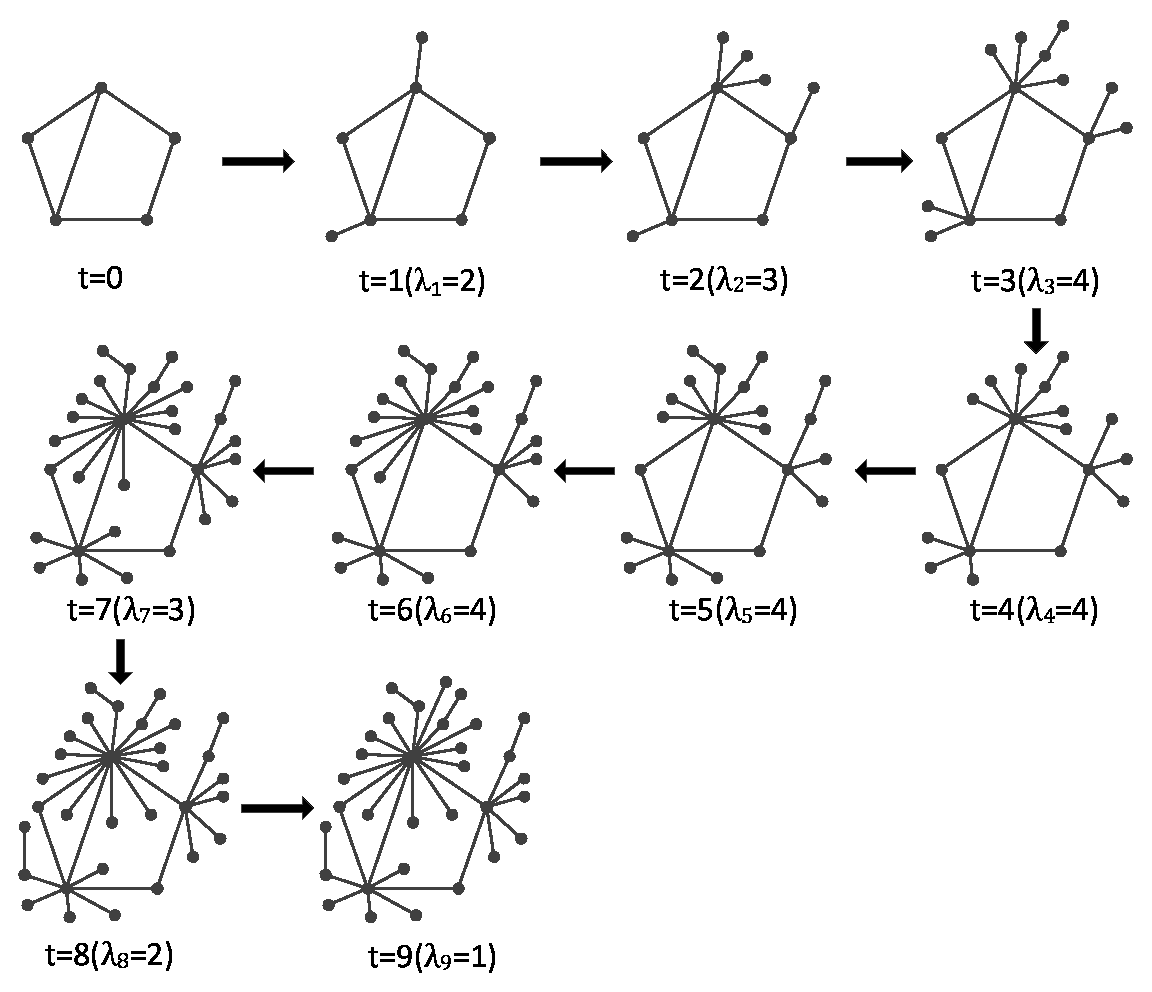
\epsfig{file=4.eps, scale=0.35}
\caption{\label{f4}Nonhomogeneous Poisson network evolution: new
vertices are generated by the rate $\lambda (t)$ and connects to
one existed vertex, the generation is terminated at time $9$.}
\end{figure}

%\begin{table}[htbp]\tiny
%\begin{center}
%\caption{\label{t3} The degree of each vertex in Fig. \ref{f4}
%($t=9$).}
%\begin{tabular}{|c|c|c|c|c|c|c|}
%\hline Degree & 1 & 2   &3 & 7 & 9 & 16\\
%\hline
%   Number  & 25  & 7  & 1  & 1 &1 &1\\
%\hline
% \end{tabular}
%\end{center}
%\end{table}

%For Fig. \ref{f4}, the number of degree $\{1, 2, 3, 6, 9, 16\}$ is
%$\{25, 7, 1, 1, 1, 1\}$,

Next, we focus on the degree distribution of the nonhomogeneous
Poisson network. Suppose that $\lambda (t)$ as Eq. \ref{e32}, and
for clarity, we assume that number of edges added each time is
fixed $\mu$ and ignore the initial network. The dynamic method is
applied to solve this issue.


Suppose that $k_{i}(t)$ is the degree of vertex $i$ at time $t$,
the the total number of added vertices is $m(t)$, then the total
degree is
\begin{equation}\footnotesize
\sum\limits_{j}k_{j}\approx2m(t)\mu
\end{equation}


The probability that an edge connects to the existed vertex $i$ is
approximated as
\begin{equation}\footnotesize
P=C_{\mu}^{1}[\Pi(k_{i})][1-\Pi(k_{i})]^{\mu-1}\approx\mu\Pi(k_{i})=\frac{k_{i}}{2m(t)}
\end{equation}

The degree growth rate of $i$ in unit time is $\lambda (t) P$, and
dynamic equation based on the continuum theory is expressed as
\begin{equation}\footnotesize
  \left\{
   \begin{aligned}
   &\frac{\partial k_{i}(t)}{\partial t} \approx\frac{k_{i}\lambda(t)}{2m(t)}\\
&k_{i}(m^{-1}(i))=\mu\\
   \end{aligned}
   \right.
  \end{equation}
where $m^{-1}(i)$ denotes the time vertex $i$ arrives, notice that
$\frac{1}{k}\partial k$$=$$\frac{\partial m(t)}{2m(t)}$, the
general solution is $k_{i}(t)$$=$$m(t)^{\frac{1}{2}}C$, and with
the substitution of the condition, the result is
\begin{equation}
k_{i}(t)=\mu[\frac{m(t)}{i}]^{\frac{1}{2}}
\end{equation}


Assuming that vertex $i$ is randomly selected from $m(t)$ vertices
and follows a homogeneous distribution, that is,
$p(i)$$=$$\frac{1}{m(t)}$, the transient degree distribution is
\begin{equation}\footnotesize
P\{k_{i}(t)<k\}=P\{i>m(t)(\frac{\mu}{k})^{2}\}=1-\frac{m(t)(\frac{\mu}{k})^{2}}{m(t)}\\
\end{equation}
the partial derivatives of $k$ is
\begin{equation}\footnotesize
P_{k}(t)=\frac{\partial P\{k_{i}(t)<k\}}{\partial
k}=2\mu^{2}k^{-3}
\end{equation}
then, the steady degree distribution is
\begin{equation}\footnotesize
P(k)=\lim\limits_{t\rightarrow\infty}P_{k}(t)=2\mu^{2}k^{-\gamma}
\end{equation}
where $\gamma$$=$$3$ and is independent of time.


From this derivation, we can see that no matter homogeneous or
nonhomogeneous the generation rate is, as long as it is
continuous, the degree distribution keeps stable, and the
different time range has no influence on the distribution.
%practically saying, even if in the war time, the topology of
%degree distribution of social network is same as in the peace
%time.



\subsection{Birth and Death Network}

The last network model is more complicated than two previous
models, which takes both the generation of vertices and their
extinctions into consideration, we call it Birth and Death Network
Model.

So far, most of network models for complex systems ignore the
degenerations of vertices, but these phenomenon really exists and
has a significant influence on the network topology. Therefore, we
should ponder both generation and degeneration. In this model, the
birth of vertices follows a Poisson process, the generation of
edges follows a Gaussian distribution, the key issue is the death
process. And in the view of practical situation, the death follows
the rule that ``The rich live while the poor die", or ``the rich
are getting richer, and the poor poorer". That is to say,
Barab\'{a}si only consider half of the Matthew effect, and we
extend it to the aspect of poor.

The death mechanism is the the crucial issue for birth and death
networks. We assume that the death time follows an exponential
distribution with parameter $\mu$, indicating that the
degeneration of old vertices is also a Poisson process. The
selection of one vertex to die follows the Matthew effect, that
is, the lower degree vertex is more likely to die. To solve
$\Gamma$, the probability of existed vertices to die, the value
convert $\widetilde{k_{i}}$ is required, that is
\begin{equation}\footnotesize
\widetilde{k_{i}}=\frac{k_{max}-k_{i}}{k_{max}-k_{min}}
\end{equation}
$\widetilde{k_{i}}$ is also said to be the poor degree, obviously,
the low degree vertex has a high value of $\widetilde{k_{i}}$.

Then, $\Gamma_{i}$ is denoted as
\begin{equation}\footnotesize
\Gamma_{i}=\frac{\widetilde{k_{i}}}{\sum
\limits_{j}\widetilde{k_{j}}}
\end{equation}
which ensures that the poor is more likely to be perished and
$\sum\limits_{i}\Gamma_{i}=1$. Then, we utilize roulette to select
the vertex to be perished. By this mechanism, the degeneration
process is confirmed.

The complete construction process is as follows:

\textbf{Initialization}: Given $N$ vertices as a nearest-neighbor
coupled networks, in which each vertex connects to its $K/2$
neighbors on the left and the right; For any pair of vertices, an
extra connection is established by the probability of $p$.


\textbf{Growth and Extinction}: Newly added vertices $i$ are
coming by the rate at $\lambda$; For each new vertex, $\eta_{i}$
edges are connected to the existing vertices. The existed vertices
are gone by the rate at $\nu$.

\textbf{Connection and Disconnection}: The probability of a newly
added vertex connected to an existing vertex is decided by
$\Pi_{k}$. The probability of an existed vertices to die is
decided by $\Gamma(k_{i})$.

\textbf{Termination}: Once time reaches $T$, the algorithm
terminates and the network is output.



We demonstrates a birth and death network evolution. The initial
network refers to Fig. \ref{f1}, and each new vertex connects to
one existed vertex, the process is displayed in Fig. \ref{f5}.

\begin{figure}[!htp]
\centering
 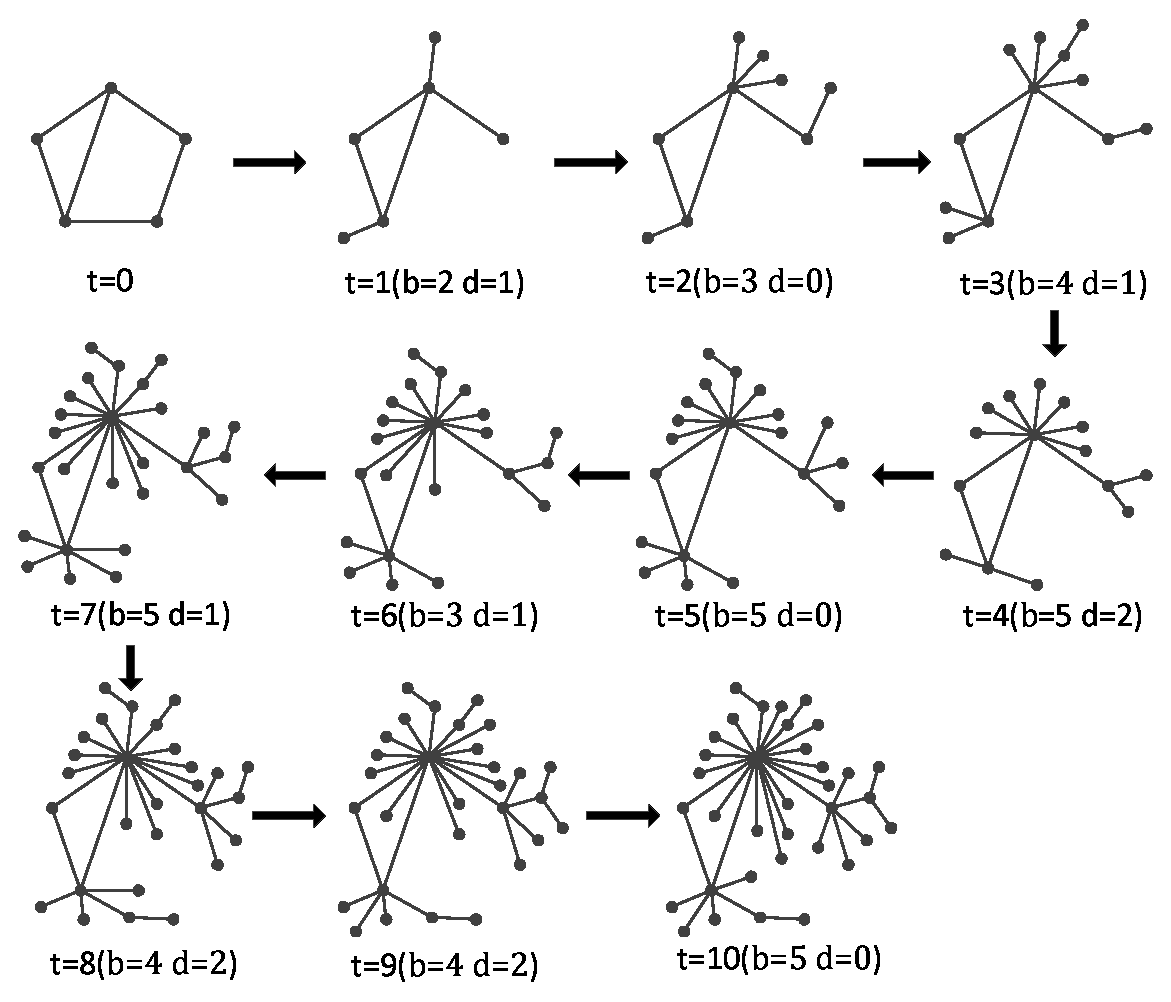
\epsfig{file=5.eps, scale=0.35}
\caption{\label{f5} Birth and death network evolution: new
vertices are generated by the rate $\lambda $ and connects to one
existed vertex, old vertices degenerate by the rate $\nu$, the
process is terminated at time $10$.}
\end{figure}

%\begin{table}[htbp]\tiny
%\begin{center}
%\caption{\label{t3} The degree of each vertex in Fig. \ref{f5}
%($t=10$).}
%\begin{tabular}{|c|c|c|c|c|c|c|}
%\hline Degree & 1 & 2   &3 & 6 & 7 & 19\\
%\hline
%   Number  & 27  & 4   & 1  & 1 &1 &1\\
%\hline
% \end{tabular}
%\end{center}
%\end{table}

From this figure, we can see that the mean generate rate
$\lambda=(2+3+4+5+5+3+5+4+4+5)/10$$=$$4$ while the degenerate rate
$\nu=(1+0+1+2+0+1+1+2+2+0)/10$$=$$1$. The low degree vertices
below $4$ are in the majority (about $91.43\%$), while high degree
vertices above $7$ are in the minority (about $5.71\%$), which is
a typical scale-free character.

%\begin{figure*}[t!]
%\centering
%\begin{minipage}[t]{0.3\linewidth}
%\centering
% 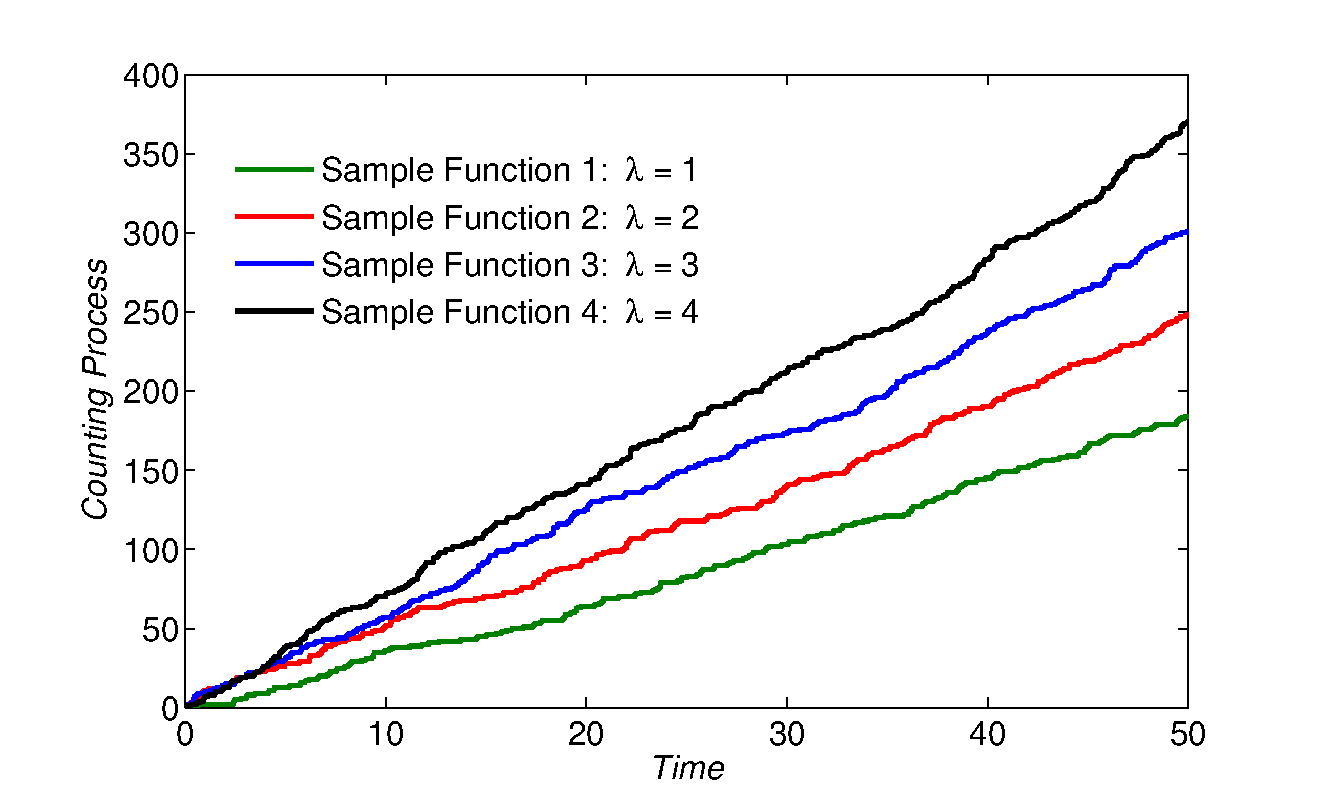
\epsfig{file=6a.eps, height=4cm, width=6cm}
%\parbox{15.5cm}{\footnotesize \hspace{2.5cm}(a) HPN}
%\end{minipage}
%\begin{minipage}[t]{0.3\linewidth}
%    \centering
% 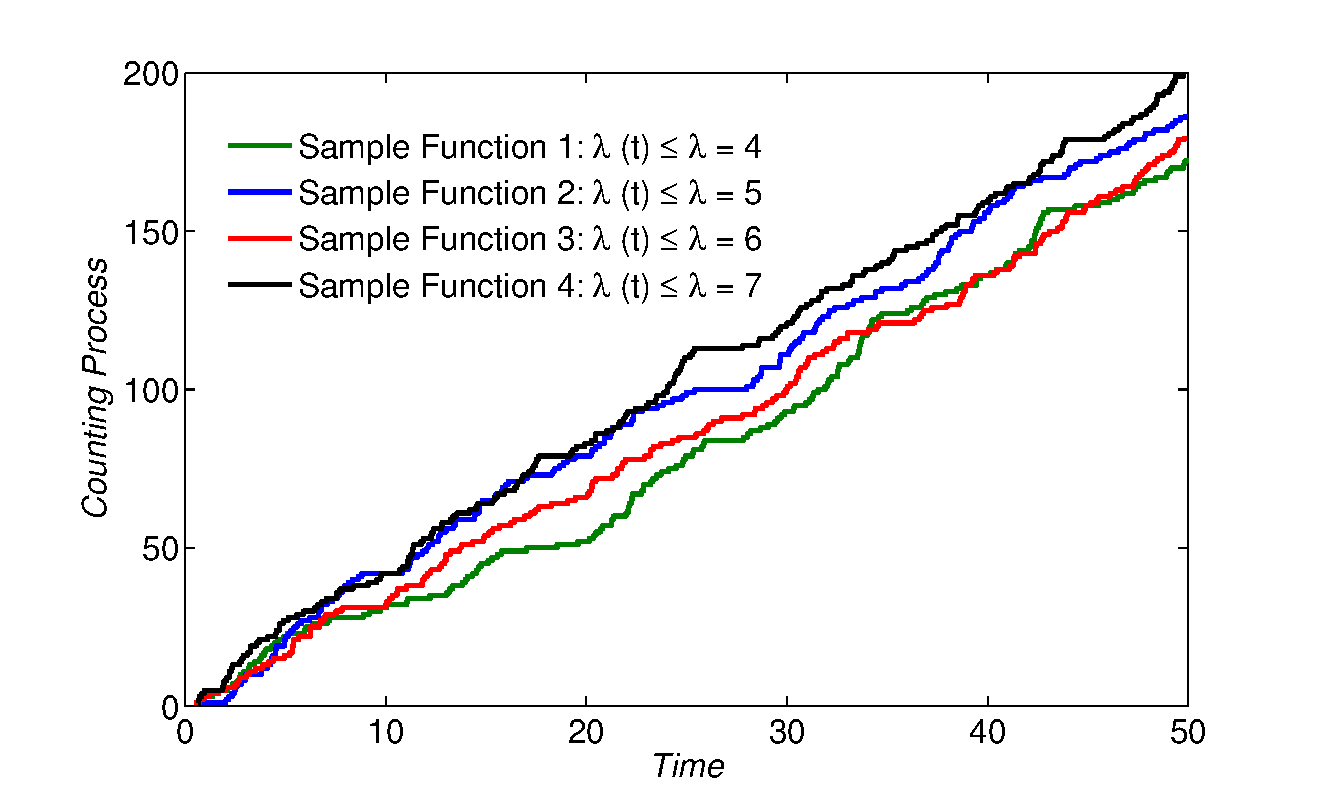
\epsfig{file=6b.eps, height=4cm, width=6cm}
% \parbox{15.5cm}{\footnotesize \hspace{2.4cm}(b) NHPN}
%\end{minipage}
%\begin{minipage}[t]{0.3\linewidth}
%    \centering
% 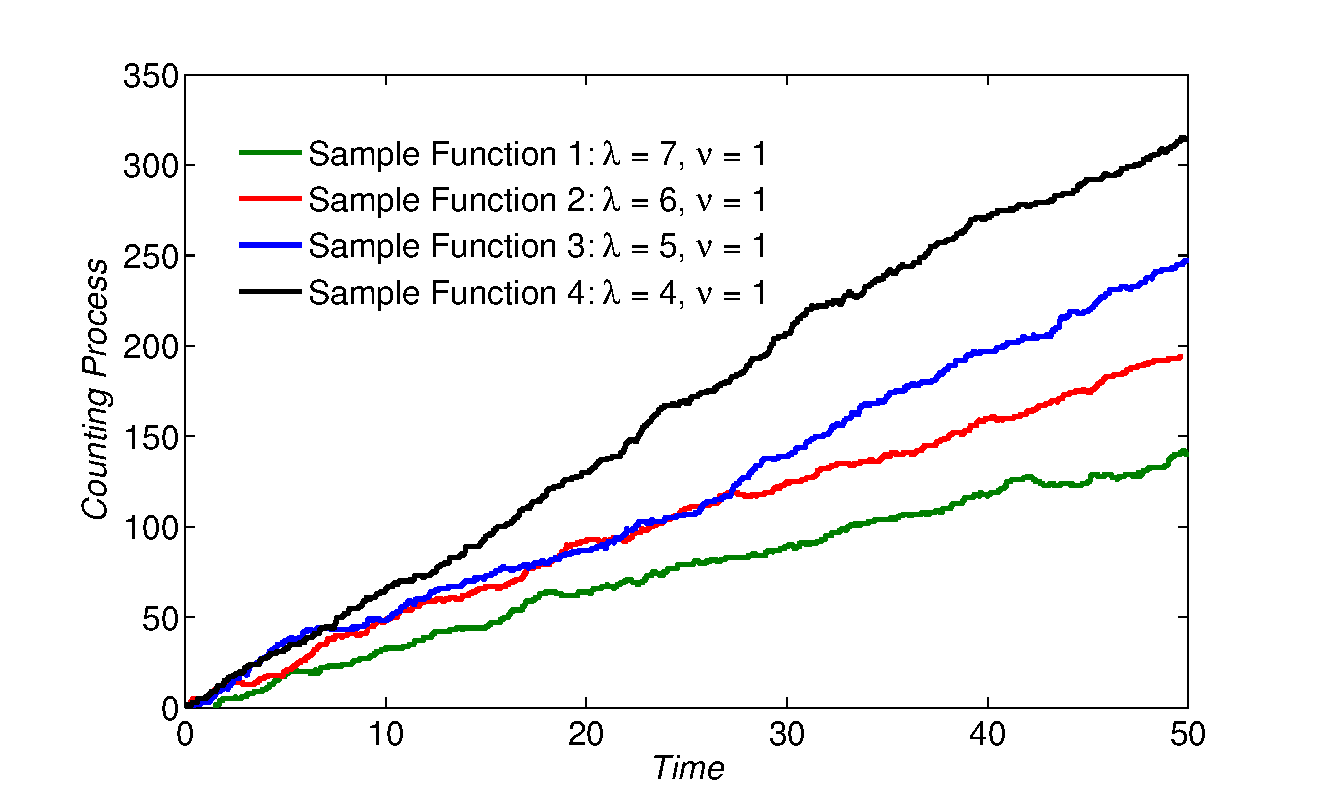
\epsfig{file=6c.eps, height=4cm, width=6cm}
% \parbox{15.5cm}{\footnotesize \hspace{2.5cm}(c) BDN}
%\end{minipage}
%\hspace{3ex}
% \caption{\label{f6} Counting processes of different models}
%\end{figure*}


%Then, we discuss the scale of birth and death network. Given
%$\lambda$ and $\nu$, the scale of network is a homogeneous markov
%chains, denoted as $\{N(t), t\geq 0\}$, which can also be
%described as a queueing system, all new vertices are regarded as
%customers and the network itself is a service system, customers
%are waiting for service, once they are connected to the existed
%vertices, they are under service, and when their services are
%done, they leave this system and are dead. Our queueing system can
%be denoted as $M/M/c/\infty/\infty$, which means the rate of
%customers follows a Poisson process, the service time follows an
%exponential distribution, $c$ servers, infinite system capacity,
%infinite customers. Then, the state transition rate matrix of
%$\{N(t), t\geq 0\}$ is
%\begin{equation}\footnotesize
%Q=\left[
%\begin{array}{p{0.3cm}<{\centering}p{1.1cm}<{\centering}p{0.1cm}<{\centering}p{0.1cm}<{\centering}p{0.1cm}<{\centering}p{1.1cm}<{\centering}p{1.1cm}<{\centering}p{0.1cm}<{\centering}}
%  -$\lambda$ & $\lambda$ \\
%   $\nu$ &-($\lambda+\nu$) &$\lambda$\\
%    % & 2$\mu$ &-($\lambda+2\mu$) & $\lambda$\\
%     &  &   &$\ddots$\\
%        &  & &  &$n\nu$ & -($\lambda+n\nu$) &$\lambda$\\
%     & & &  & &n$\nu$ & -($\lambda+n\nu$) &$\lambda$\\
%       & & &  & & &  $\ddots$\\
%   \end{array}
%\right]. \nonumber
%\end{equation}
%
%
%
%
%The state space of $\{N(t), t\geq 0\}$ is $E=\{0, 1, 2, ...\}$,
%indicating that the scale of network, and $p(t)$, the probability
%of the scale of network at time $t$, satisfies the Fokker-Planck
%equation, that is
%\begin{equation}\label{e41}\footnotesize
%\begin{aligned}
% \left\{
%   \begin{aligned}
%   &p'_{j}(t)=-(\lambda+j\nu)p_{j}(t)+\lambda p_{j-1}+(j+1)\nu p_{j+1}, 0< j< c\\
%   &p'_{j}(t)=-(\lambda+c\nu)p_{j}(t)+\lambda p_{j-1}+c\nu p_{j+1}, \hspace{0.8cm} j\geq c\\
%&p'_{0}(t)=-\lambda p_{0}(t)+\nu p_{1}(t)\\
%   \end{aligned}
%   \right.
%\end{aligned}
%\end{equation}
%let $p_{j}$$=$$\lim\limits_{t\rightarrow \infty}p_{j}(t)$, there
%are two situations:
%
%\noindent(1) If $\lambda$$ >$$c\nu$, $p_{j}=0$;
%
%\noindent(2) If $\lambda$$ <c$$\nu$, then,
%\begin{equation}\label{e42}\footnotesize
%p_{j}=\begin{aligned}
% \left\{
%   \begin{aligned}
%   & \frac{1}{j!}\rho^{j}p_{0}, \hspace{1.4cm}0< j< c\\
%   & \frac{1}{c!c^{j-c}}\rho^{j}p_{0}, \hspace{0.8cm}j\geq c\\
%   \end{aligned}
%   \right.
%\end{aligned}
%\end{equation}
%where
%$p_{0}$$=$$[\sum\limits_{t=0}^{c-1}\frac{\rho^{j}}{j!}+\frac{c\rho^{j}}{p_{0}}]^{-1}$.
%
%
%From this solution, we can see that if $\lambda >c\nu$, the scale
%of network is unstable and keeps growing all the time, else if
%$\lambda <c\nu$, the average scale of network is
%\begin{equation}\label{e43}\footnotesize
%N=\sum\limits_{k=0}^{\infty}jp_{j}=\rho+\frac{\rho^{c+1}}{cc!(1-\frac{\rho}{n})^{2}}p_{0}
%\end{equation}
%which indicates, under this situation, $t$$\rightarrow$$ \infty$,
%the scale of network is stable. However, the input rate is usually
%higher than the output (including our simulation), in that case,
%for most of birth and death network, the steady distribution does
%not exist.

The degree distribution of birth and death network is different
from the other two and more complex, the dynamic method and
probabilistic approach cannot obtain the solution, we still try to
work it out and require further study.

\section{Simulation and Analysis}
In this section, we focus on modeling process and displaying the
statistical degree distribution of proposed network models,
besides, the robustness and vulnerability simulation is carried
out. For simplicity, HPN denotes the Homogeneous Poisson Network,
NHPN denotes the NonHomogeneous Poisson Network and BDN denotes
the Birth and Death Network in following subsections.



\begin{figure*}[t!]
\centering
\begin{minipage}[b]{0.3\linewidth}
\centering
 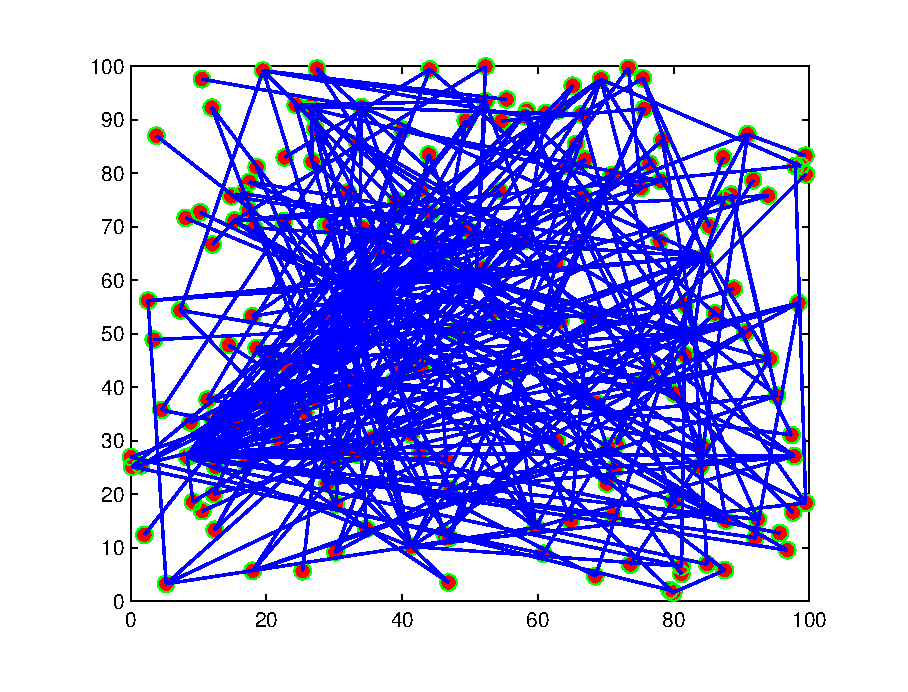
\epsfig{file=7a.eps, scale=0.4}
\parbox{15.5cm}{\footnotesize \hspace{2.5cm}(a) HPN}
\end{minipage}
\begin{minipage}[b]{0.3\linewidth}
    \centering
 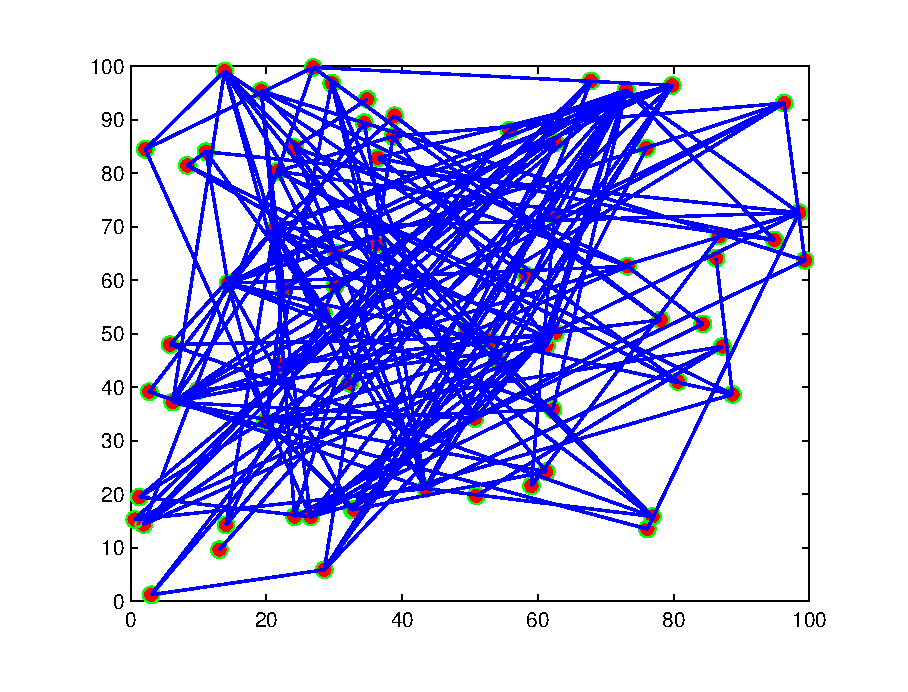
\epsfig{file=7b.eps, scale=0.4}
 \parbox{15.5cm}{\footnotesize \hspace{2.4cm}(b) NHPN}
\end{minipage}
\begin{minipage}[b]{0.3\linewidth}
    \centering
 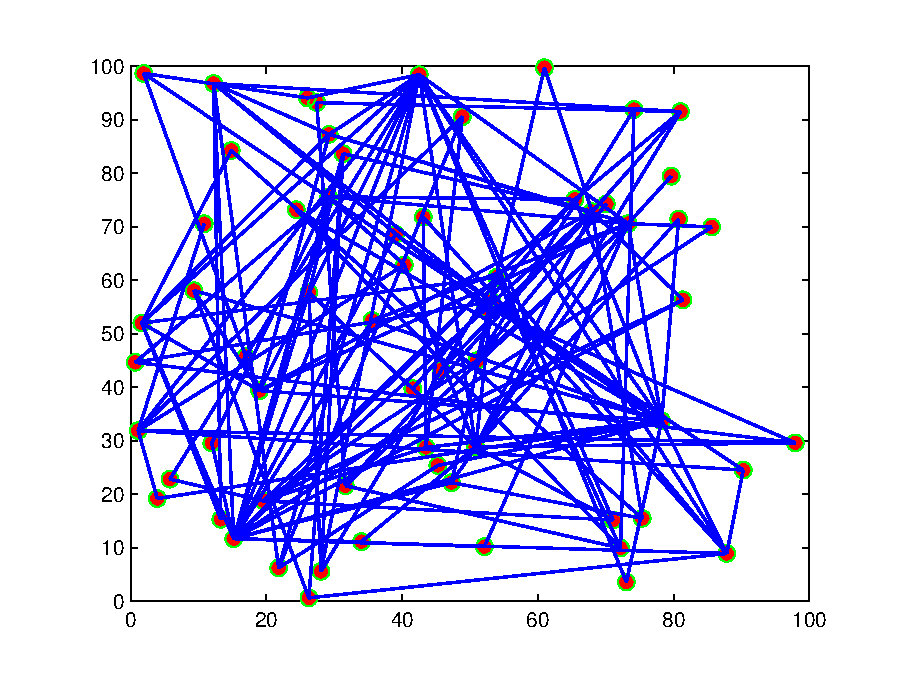
\epsfig{file=7c.eps, scale=0.4}
 \parbox{15.5cm}{\footnotesize \hspace{2.5cm}(c) BDN}
\end{minipage}
\hspace{3ex}
 \caption{\label{f7} Illustration for three different networks: initial networks all start with
$10$ nodes, each node connects to its two neighbors on the left
and right, with the probability $0.2$ to add a path to the other
node. The setting is: (a) $\lambda=4$, (b) $\lambda (t) \leq
\lambda =4$, (c) $\lambda=4$, $\mu=1$. The termination time
$T_{max}=50$.}
\end{figure*}


\subsection{Network Modeling}
Modeling of network is the foundation of our simulation, and the
random process is the linchpin of modeling, therefore, we mainly
describe the simulation of random processes in this subsection.



%\begin{figure}[!htp]
%\centering
% 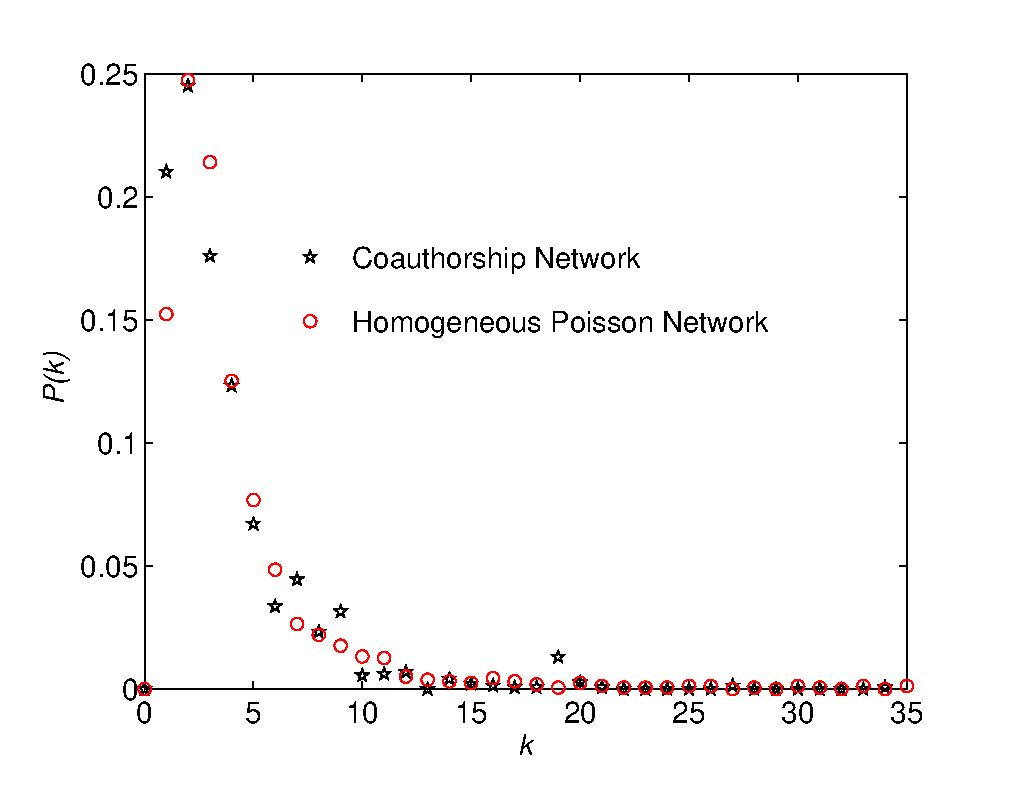
\epsfig{file=xxx.eps, scale=0.5}
%\caption{\label{f8} The sample of deviations from a mathematical
%Power-law. The continuous line is a mathematical Power-law with
%$\gamma =3$, and discrete points denote the empirical data.}
%\end{figure}


The key of a HPN is to simulate a poisson process with $\lambda$,
in other words, a mutually independent exponential distribution
random sequence with expectation $\frac{1}{\lambda}$ is required.
Then, our method is as follows:

\noindent$\diamond$ set the value of $\lambda$
and $T_{max}$;

\noindent$\diamond$ generate exponential distribution random
values with $\lambda$,

 denoted as $t_{i}$

\noindent$\diamond$ if cumulative time $T_{i}\leq T_{max}$, let
$T_{i}=T_{i}+t_{i}$, else output

the temporal series.

%By these steps, we can obtain a temporal series for the Poisson
%process, Fig. \ref{f6} (a) show examples that vertices growing
%with time by different rate $\lambda$.

The temporal series of a NHPN is produced by the rarefaction
method, that is, assuming $\lambda (t)\leq \lambda$, where
$\lambda$ is a constant, $\{t_{1}, t_{2}, \cdots\}$ is the
temporal series of a homogeneous Poisson process with $\lambda$,
for each $t_{i}$, with the probability $\frac{\lambda
(t_{i})}{\lambda}$ to save and $1-\frac{\lambda (t_{i})}{\lambda}$
to abandon, then, the saved temporal series $\{t_{1}', t_{2}',
\cdots\}$ follows the nonhomogeneous Poisson with $\lambda (t)$.
The detailed process is as follows:

\noindent$\diamond$ Produce the temporal series with parameter
$\lambda$, denoted as

$\{t_{1}, t_{2}, \cdots\, t_{n}\}$;

\noindent$\diamond$ Generate a random number $r_{i}$, if
$r_{i}\leq \frac{\lambda (t_{i})}{\lambda}$, $t_{i}$ is saved,

else $t_{i}$ is abandoned;

\noindent$\diamond$ For those saved $t_{i}$, remark them as
$\{t_{1}', t_{2}', \cdots\, t_{k}'\}$ and

output.



%Vertices growth with time by different $\lambda$ and $\lambda (t)$
%follows Eq. \ref{e32} is displayed in Fig. \ref{f6} (b).

The BDN is different from other two, we employ a queuing system
$M/M/1/\infty/\infty$, the temporal series of generation and
degeneration both follow exponential distribution random sequences
with expectation $\frac{1}{\lambda}$ and $\frac{1}{\nu}$,
respectively, the system decides serve the vertex by the rule ``
poorer die" with rate $\nu$, and records the leaving time. The
detailed process is as follows:

\noindent$\diamond$ Produce the temporal series with parameter
$\lambda$, denoted as

 $\{t_{1}, t_{2}, \cdots\, t_{n}\}$;

\noindent$\diamond$ The system serves the vertices by the rate
$\nu$, records their

leaving time, $\{T_{1}, T_{2},  \cdots\, T_{k}\}$;

\noindent$\diamond$ When $T_{max}$ is reached, output the temporal
series.


%Fig. \ref{f6} (c) shows an example of the birth and death process
%with variable $\lambda$ and constant $\nu$.


Based on these counting processes, we display three network models
shown in Fig. \ref{f7}. %The three initial networks all starts with
%$10$ nodes, each node connects to its two neighbors on the left
%and right and has the probability $0.2$ to add a path to the other
%node. The construction processes work as mentioned before. Here,
%for clarity and simplicity, we display three typical networks for
%each model, with a $\lambda=4$ for a homogeneous Poisson network,
%a $\lambda (t) \leq \lambda=4$ follows Eq. \ref{e32} for a
%nonhomogeneous Poisson network, and a $\lambda=4$, $\nu=1$ for a
%birth and death network. The termination time all sets as $50$.
%Then, the results show in Fig. \ref{f7}.




\subsection{Degree Distribution}
Degree is a simple but significant character for a single vertex
in network, and the degree distribution is the most important
property and topology for complex networks. In this section, we
use the statistical method to analyze degree distribution and
obtain a degree exponent from empirical data.


As we know, the degree distribution of most scale free networks
including our proposed models obeys the Power-law distribution,
which can be mathematically denoted as:
\begin{equation}\label{e46}\footnotesize
y=\beta x^{-\gamma}
\end{equation}
where $\beta$ is a normalization, and $\gamma$ the power law
exponent. %Obviously, the Power-law distribution is highly
%nonhomogeneous, shown in figure, those high degree vertices called
%``hub" are always in the minority, and those low degree the
%majority. And when the Power-laws are employed to denote degree
%distribution, the $\gamma$ is typically positive, implying that
%with the increase of $x$, the value of $y$ drops.

In this section, we record degrees of three different models in
multiple situations and obtain their degree distributions.
Discrete empirical data, as circles in Fig. \ref{f8}, are only
approximations of continuous mathematical Power-laws in line. The
reason for deviations of empirical data is that the process of
construction of network is much more complex than a simple
Power-law. The task for us is to employ a simple Power-law to more
precisely describe the data, thus we need to remove those complex
factors as noisy data. There are many proposed algorithm to solve
this issue, such as the logarithmic binning \cite{jeong1},
\cite{sta}, maximum likelihood estimation \cite{h}, \cite{aa} and
so on \cite{vi}, here, we apply a numerical method.


From Fig. \ref{f8}, we can see that, for the large degree $k$, the
deviation from the mathematical value is obvious. These tail
values are often caused by the statistical nature of the empirical
distribution, it appears that, at large $k$, the number of
vertices are one or zero, which causes noticeable noises. To get
rid of them, we set a noise threshold $N$ for the data, we remove
$Nt$ values from the empirical data as the statistical noise. For
example, for a data set with $1000$ points, if $N=0.005$, that
means we need to remove $5$ highest degree from this data as
noise, see tail noises in red in Fig. \ref{f8}. The value of $N$
varies with different networks to remove the long tail, generally,
$0.5\%$ to $2\%$ in this paper. In addition, since the connection
follows a Gauss distribution $\eta \sim N(\mu, \sigma^{2})$, the
value of $k$ below $\mu+\sigma$ also leads to noticeably noisy
appearance, therefore, these points are also removed, see head
noises in black in Fig. \ref{f8}.
\begin{figure}[!htp]
\centering
 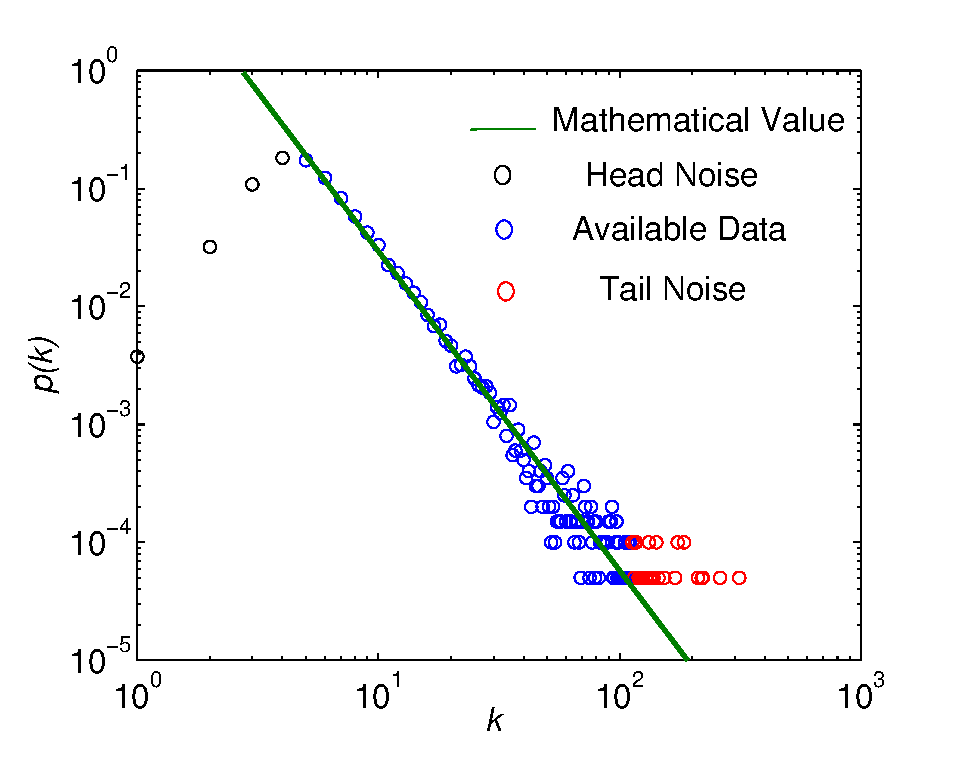
\epsfig{file=8.eps, scale=0.35}
\caption{\label{f8} The sample of deviations from a mathematical
Power-law. The continuous line is a mathematical Power-law with
$\gamma =3$, and discrete points denote the empirical data.}
\end{figure}



After noises are removed, the line fitting is required. Assuming
that the empirical data follows Eq. \ref{e46}, as we operate in
log coordinate, the equation is logged as:
\begin{equation}\label{e47}\footnotesize
A\left(
\begin{array}{p{0.35cm}<{\centering}p{0.35cm}<{\centering}}
 $x_{1}$\\
 $ x_{2}$\\
   \end{array}
\right)=b
\end{equation}
where $A$$=$$(\log x, 1)$, $x_{1}$$=$$-\gamma$, $x_{2}$$=$$\log
\beta$, $b$$=$$\log y$.


\begin{table*}\tiny
\begin{center}
\caption{\label{tx} Degree exponents for three kinds of networks
with different arguments}.
\begin{tabular}{|c|c|c|c|c|c|c|c|c|c|c|c|c|c|c|c|c|c|}
 \hline
   \multicolumn{6}{|c|}{HPN}&\multicolumn{6}{c|}{NHPN}  &\multicolumn{6}{c|}{BDN}\\
   \hline
\multicolumn{2}{|c|}{$\mu=10$}&\multicolumn{2}{c|}{$\lambda=4$}  &\multicolumn{2}{c|}{$\lambda=4$}&\multicolumn{2}{c|}{$\mu=10$}&\multicolumn{2}{c|}{$\lambda=4$}  &\multicolumn{2}{c|}{$\lambda=4$}&\multicolumn{2}{c|}{$\mu=10$}&\multicolumn{2}{c|}{$\lambda=4$}  &\multicolumn{2}{c|}{$\lambda=4$}\\
 \multicolumn{2}{|c|}{$t=1000$}&\multicolumn{2}{c|}{$t=1000$}  &\multicolumn{2}{c|}{$\mu=10$}&\multicolumn{2}{c|}{$t=1000$}&\multicolumn{2}{c|}{$t=1000$}  &\multicolumn{2}{c|}{$\mu=10$}&\multicolumn{2}{c|}{$t=1000$}&\multicolumn{2}{c|}{$t=1000$}  &\multicolumn{2}{c|}{$\mu=10$}\\
 \hline
$\lambda$ &$\gamma$& $\mu$ &$\gamma$&$t$&$\gamma$& $\lambda$&$\gamma$&$\mu$ &$\gamma$&$t$&$\gamma$&$\lambda$ &$\gamma$&$\mu$ &$\gamma$&$t$&$\gamma$\\
 \hline
  4  &2.7 &10&2.9&1000&2.9&4  &2.8 &10&3.0&1000&2.9 &4  & 3.0&10&2.9&1000&2.9\\
 \hline
 6 &2.8&20&2.8&2000&2.8&6 &3.0&20&2.8&2000&2.7&6 &2.9&20&2.9&2000&2.8\\
 \hline
 8&2.8&30&2.8&3000&2.9& 8&2.9&30&3.0&3000&2.8 & 8&3.0&30&2.8&3000&2.8\\
 \hline
 10 &2.9&40&2.7&4000&2.9&10 &2.8&40&2.8&4000&2.8&10 &3.0&40&3.0&4000&2.8\\
 \hline
  12 &2.9&50&2.8&5000&3.0& 12 &2.8&50&2.9&5000&3.0 &12 &2.8 &50&3.1&5000&2.8\\
 \hline
\end{tabular}
\end{center}
\end{table*}


%Once empirical values $\log x$, $\log y$ are obtained, we employ
%them in Eq. \ref{e47} and get the solutions
%$\overline{x}$$=$$(x_{1}, x_{2})$. For these solutions, the
%Euclidean norm for vectors is applied to measure the distance from
%$\overline{x}$ to real solution $x$, which is also known as 2-norm
%or squared error and denoted as
%$\|r\|_{2}=\sqrt{r_{1}^{2}+r_{2}^{2}+\cdots r_{n}^{2}}$.

To get the best fitting line, we need to seek for the least
squared error, equationally, that is
\begin{equation}\label{e48}\footnotesize
\begin{aligned}
 \left\{
   \begin{aligned}
   & \min \|b-A\overline{x}\|_{2}\\
   & s.t. A^{T}A\overline{x}=A^{T}b\\
   \end{aligned}
   \right.
\end{aligned}
\end{equation}
where $\overline{x}$$=$$(x_{1}, x_{2})$. $x_{1}$ in solution
$\overline{x}$ for Eq. \ref{e48} is the slope of the best fitting
line. With this argument, we can determine the plot for the degree
distribution of a network.


\begin{figure*}[t!]\tiny
\centering
\begin{minipage}[b]{0.3\linewidth}
\centering
 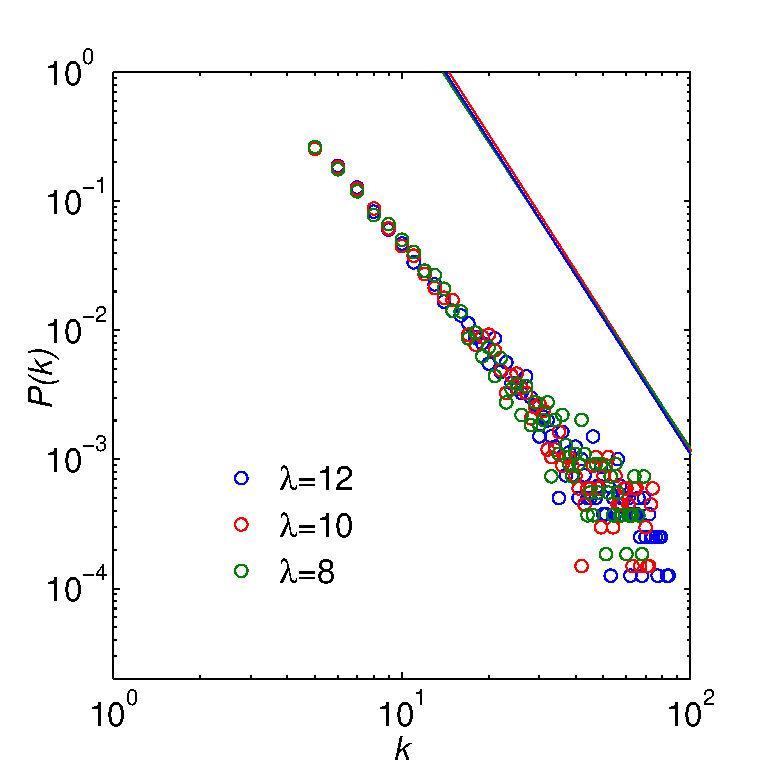
\epsfig{file=9a.eps, height=4cm, width=5.5cm}
\parbox{15.5cm}{\small \hspace{2.5cm}(a)}
\end{minipage}
\begin{minipage}[b]{0.3\linewidth}
    \centering
 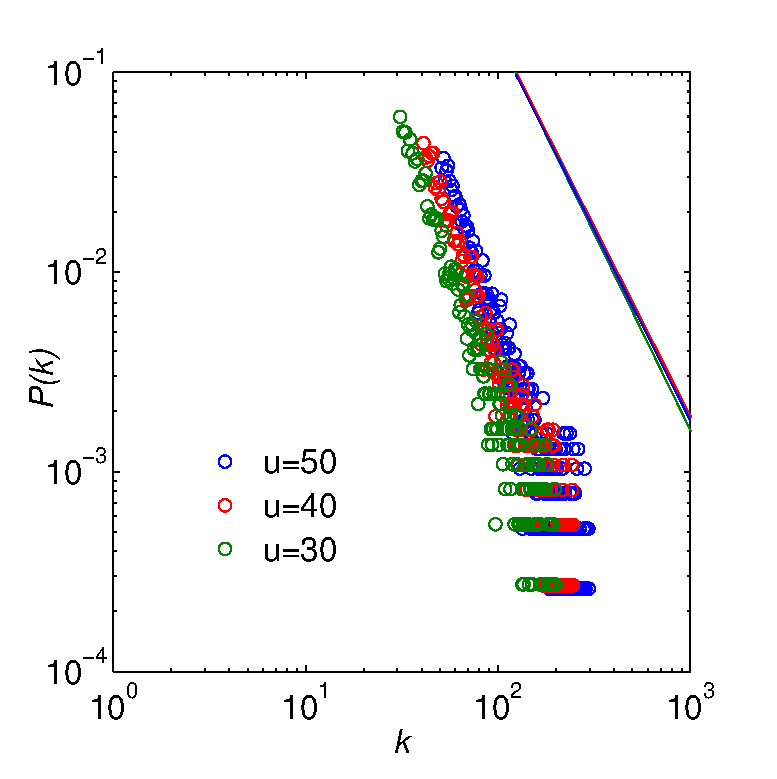
\epsfig{file=9b.eps, height=4cm, width=5.5cm}
 \parbox{15.5cm}{\small \hspace{2.5cm}(b)}
\end{minipage}
\begin{minipage}[b]{0.3\linewidth}
    \centering
 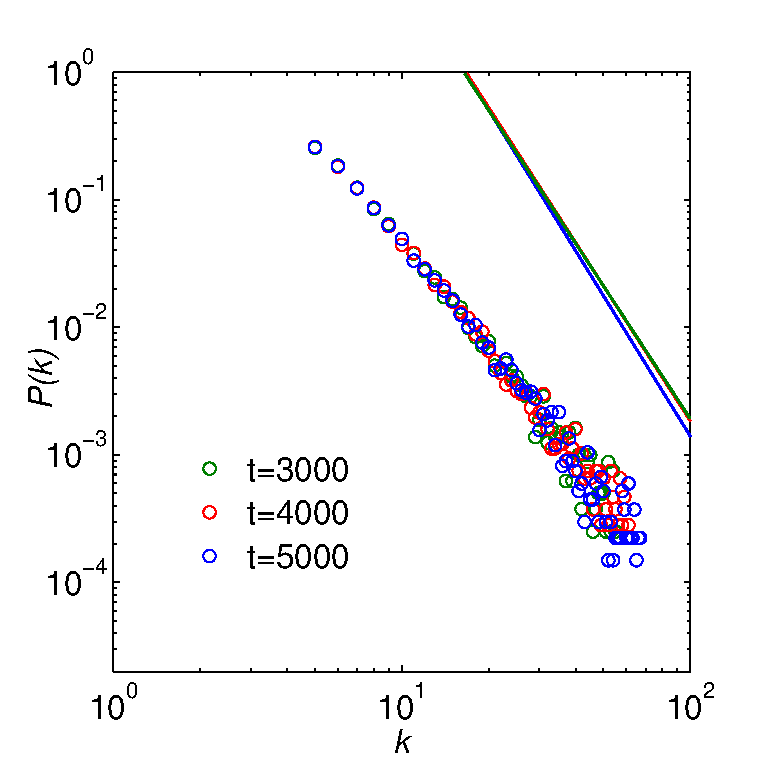
\epsfig{file=9c.eps, height=4cm, width=5.5cm}
 \parbox{15.5cm}{\small \hspace{2.5cm}(c) }
\end{minipage}
\hspace{3ex}
 \caption{\label{f9} Degree distributions of HPNs with different arguments in logarithmic coordinates. Arguments are setting as: (a) $\mu$$==$$10$, $t$$==$$1000$, (b) $\lambda$$==$$4$, $t$$=$$1000$, (c) $\lambda$$=$$4$, $\mu$$=$$10$.}
\centering
\begin{minipage}[b]{0.3\linewidth}
\centering
 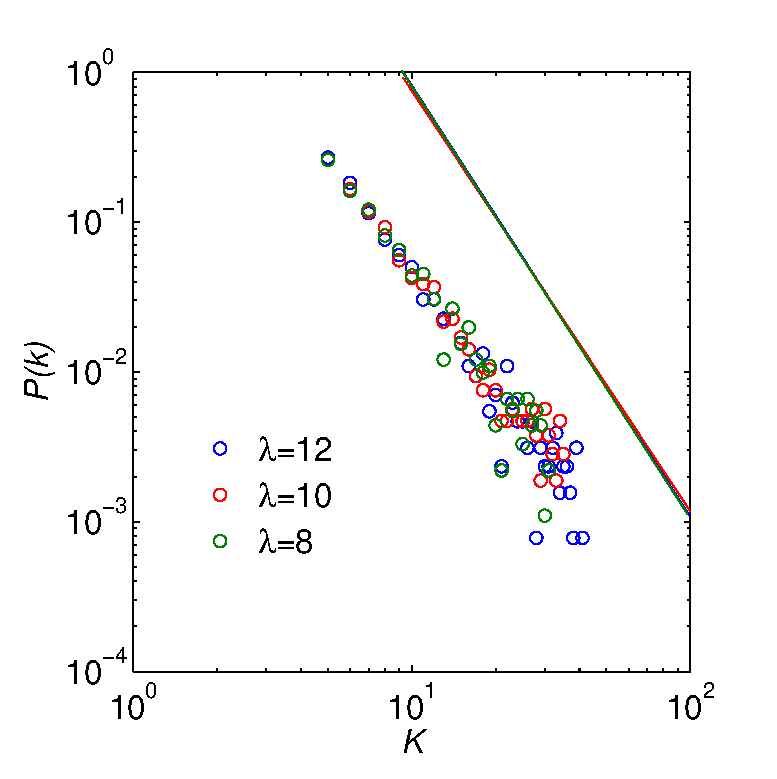
\epsfig{file=10a.eps, height=4cm, width=5.5cm}
\parbox{15.5cm}{\small \hspace{2.5cm}(a)}
\end{minipage}
\begin{minipage}[b]{0.3\linewidth}
    \centering
 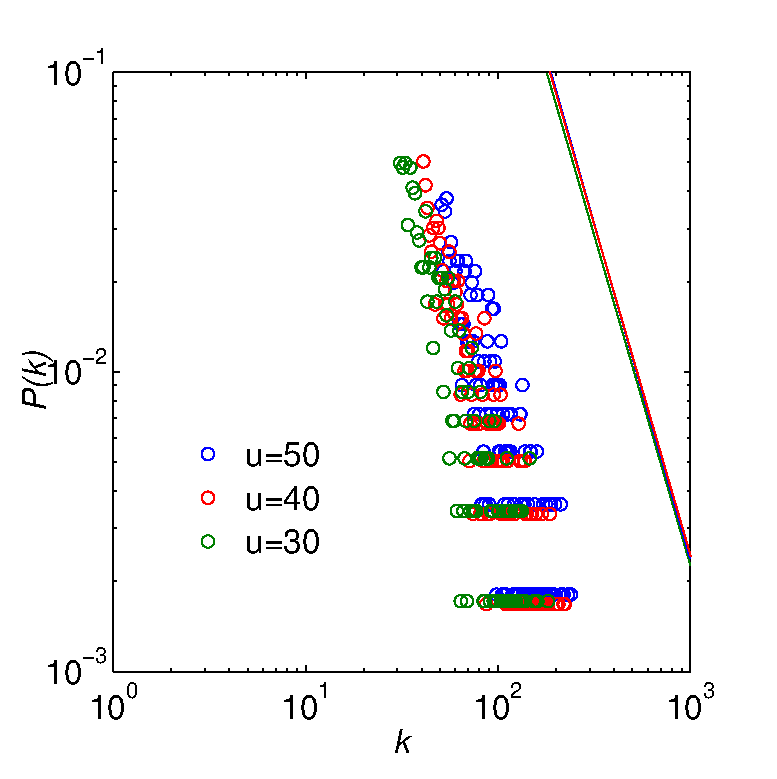
\epsfig{file=10b.eps, height=4cm, width=5.5cm}
 \parbox{15.5cm}{\small \hspace{2.5cm}(b)}
\end{minipage}
\begin{minipage}[b]{0.3\linewidth}
    \centering
 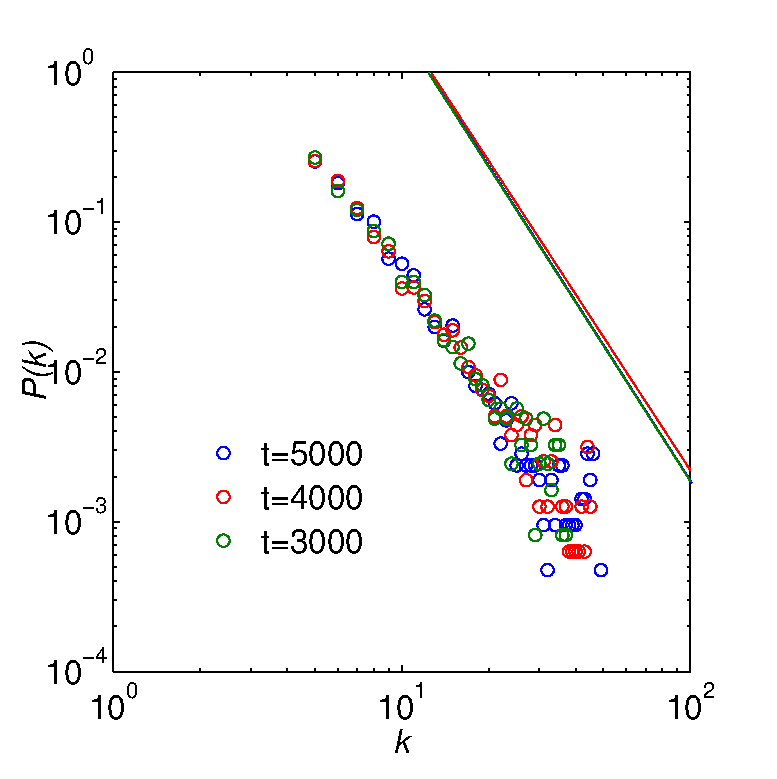
\epsfig{file=10c.eps, height=4cm, width=5.5cm}
 \parbox{15.5cm}{\small \hspace{2.5cm}(c)}
\end{minipage}
\hspace{3ex}
 \caption{\label{f10} Degree distributions of NHPNs with different arguments in logarithmic coordinates. Arguments are setting as: (a) $\mu$$==$$10$, $t$$==$$1000$, (b) $\lambda$$==$$4$, $t$$=$$1000$, (c) $\lambda$$=$$4$, $\mu$$=$$10$.}
\centering
\begin{minipage}[b]{0.3\linewidth}
\centering
 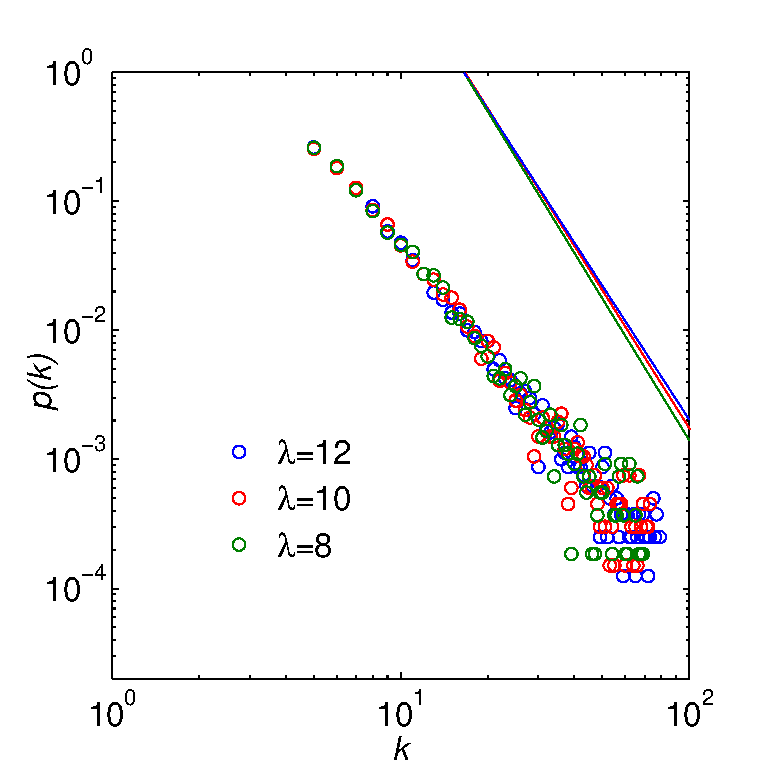
\epsfig{file=11a.eps, height=4cm, width=5.5cm}
\parbox{15.5cm}{\small \hspace{2.5cm}(a) }
\end{minipage}
\begin{minipage}[b]{0.3\linewidth}
    \centering
 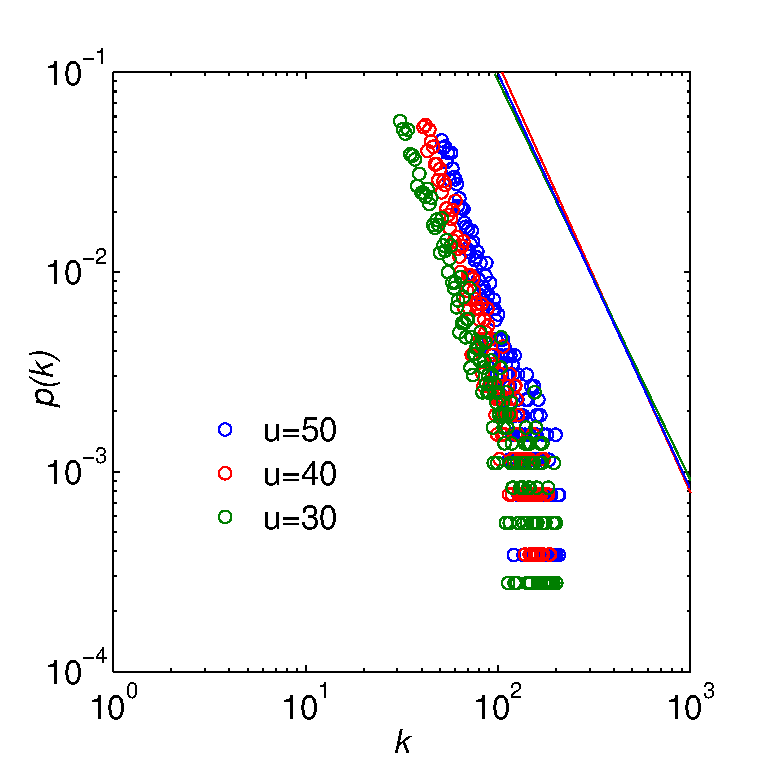
\epsfig{file=11b.eps, height=4cm, width=5.5cm}
 \parbox{15.5cm}{\small \hspace{2.5cm}(b)}
\end{minipage}
\begin{minipage}[b]{0.3\linewidth}
    \centering
 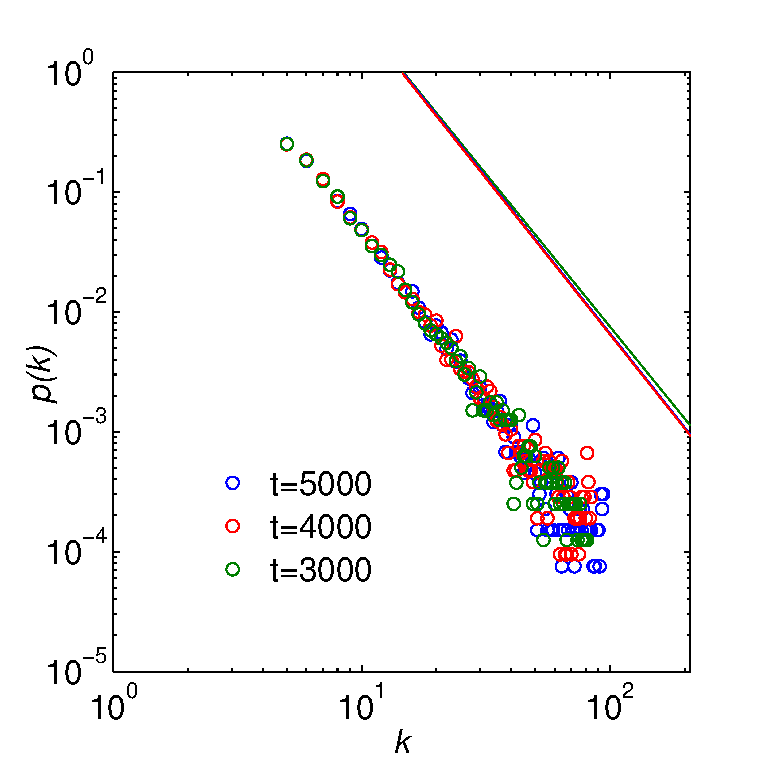
\epsfig{file=11c.eps, height=4cm, width=5.5cm}
 \parbox{15.5cm}{\small \hspace{2.5cm}(c)}
\end{minipage}
\hspace{3ex}
 \caption{\label{f11} Degree distributions of BDNs with different arguments in logarithmic coordinates. Arguments are setting as: (a) $\mu$$==$$10$, $t$$==$$1000$, (b) $\lambda$$==$$4$, $t$$=$$1000$, (c) $\lambda$$=$$4$, $\mu$$=$$10$.}
\end{figure*}

By utilizing this method, we plot degree distributions for three
network models in double logarithmic coordinates and obtain the
slope, which is also the degree exponent. In this simulation, we
mainly consider three variables: the input rate, connection and
time. Specifically, for HPN $\lambda$, $\mu$ and $t$ are measured;
for NHPN, $\lambda(t)$$\leq$$\lambda$, $\mu$ and $t$ are measured;
for BDN, $\lambda$, $\nu_{d}$$=$$\frac{1}{3}$, $\mu$ and $t$. One
argument is changed while other two are constant, so that we can
observe whether the degree exponent has a relationship with these
arguments. Detail argument settings and results of degree
exponents are listed in Tab. \ref{tx}. The table gives three
network HPN, NHPN and BDN, for each, we increase $\lambda$ from
$4$ to $12$, $\mu$ from $10$ to $50$ and $t$ from $1000$ to
$5000$, the corresponding degree exponents $\gamma$ are also
listed.


From this table, we can draw the conclusion that, for all three
networks, the value range of degree exponents lies in $[2.7,
3.0]$, which is independent of $\lambda$, $\mu$ and $t$. %In the
%strict sense, although the value fluctuates from one to another,
%but it appears no direct relationship with the arguments, and the
%reason for fluctuation is artificial errors of removal of noise.

\begin{figure*}[t!]
\centering
\begin{minipage}{0.3\linewidth}
\centering
 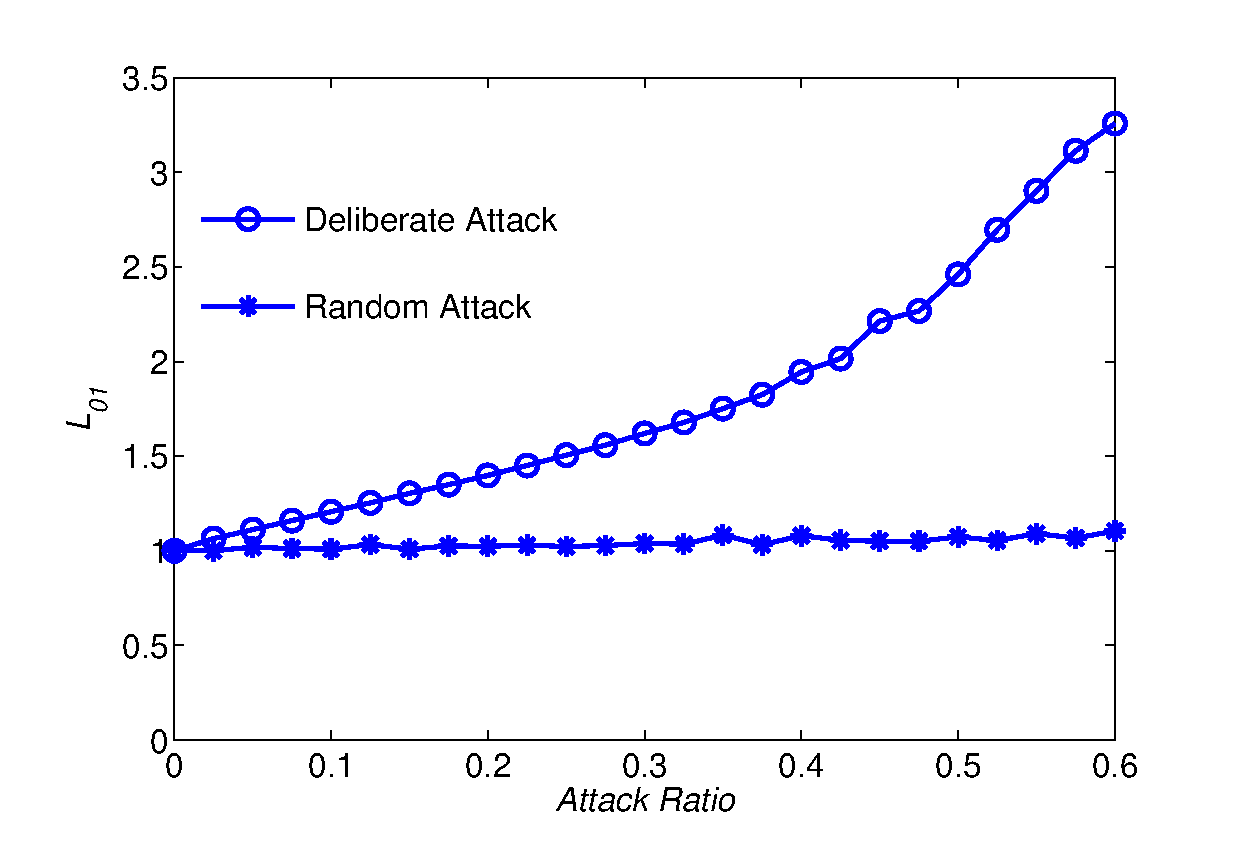
\epsfig{file=12a.eps, height=4cm, width=6cm}
\parbox{15.5cm}{\footnotesize \hspace{2.5cm}(a) HPN}
\end{minipage}
\begin{minipage}{0.3\linewidth}
    \centering
 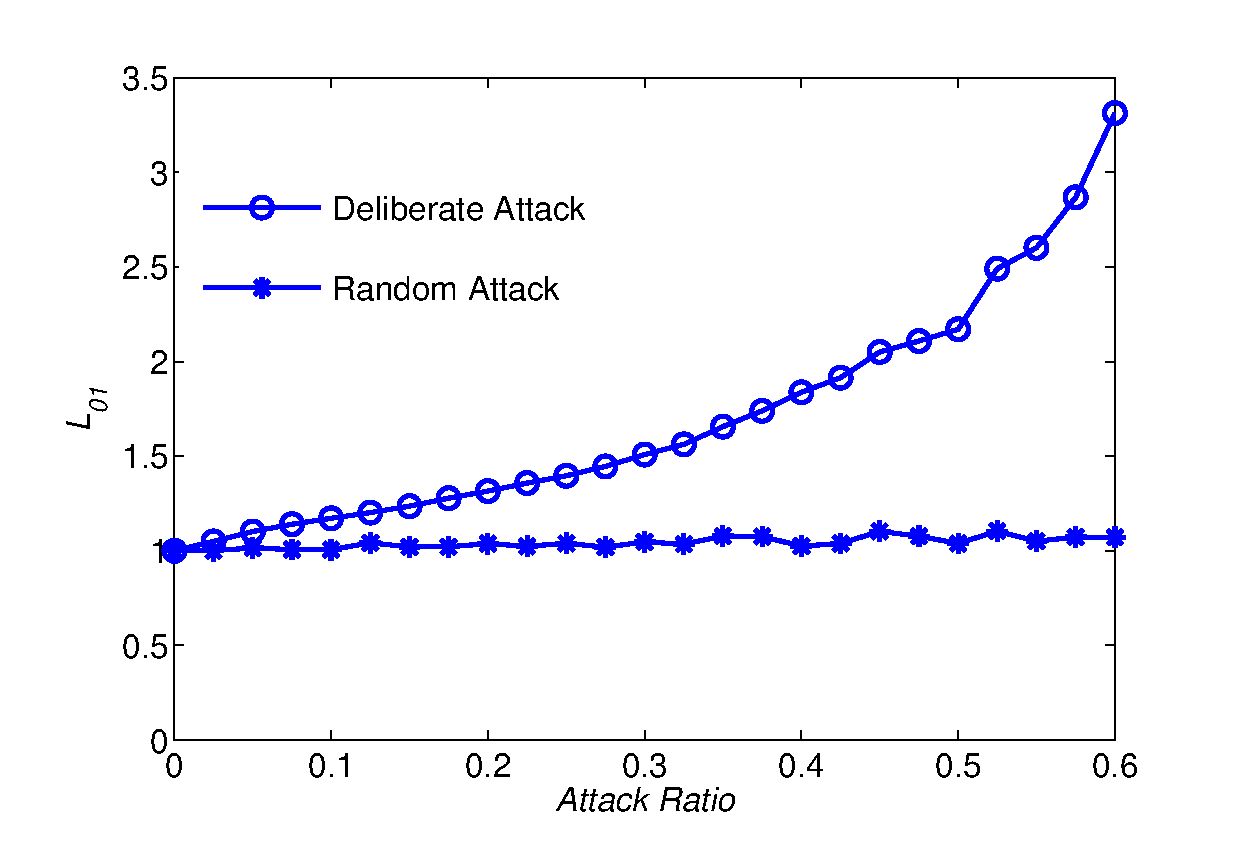
\epsfig{file=12b.eps, height=4cm, width=6cm}
 \parbox{15.5cm}{\footnotesize \hspace{2.3cm}(b) NHPN.}
\end{minipage}
\begin{minipage}{0.3\linewidth}
    \centering
 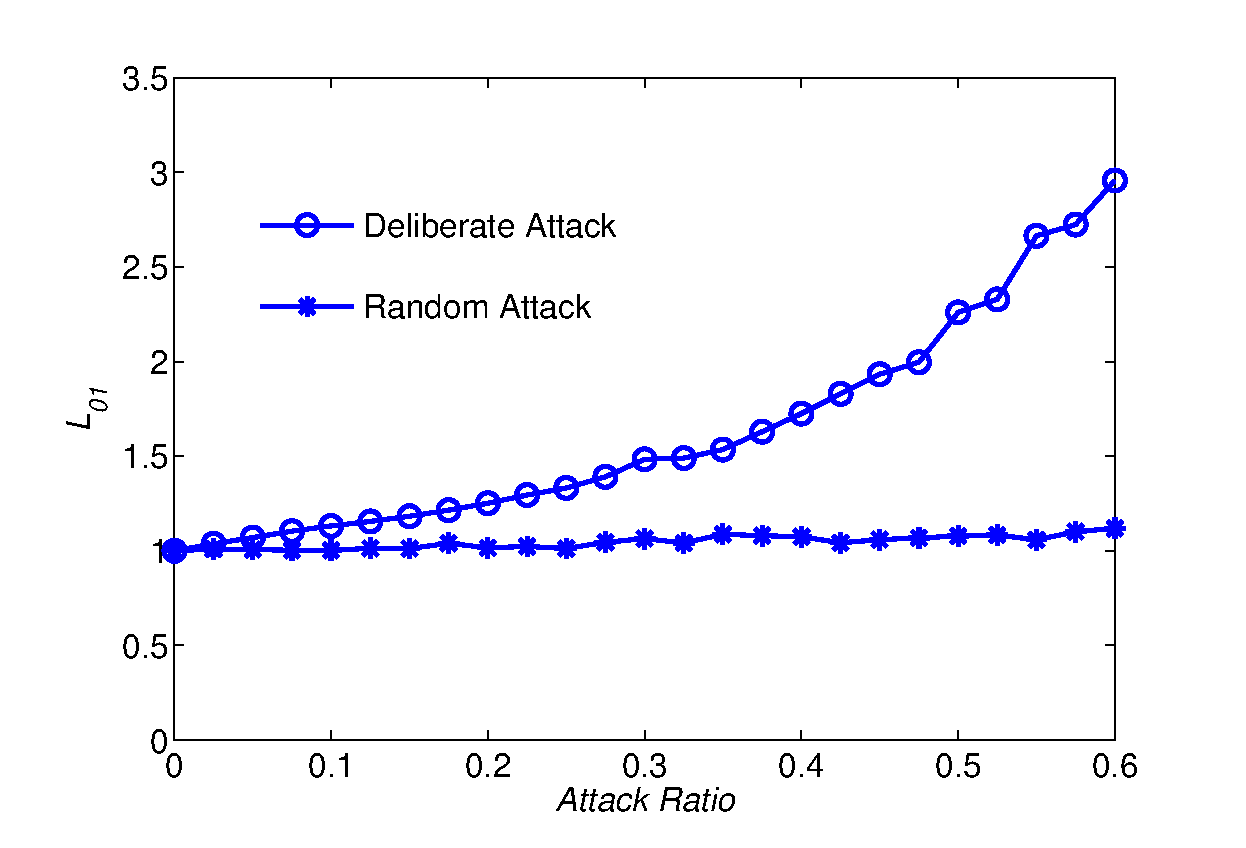
\epsfig{file=12c.eps, height=4cm, width=6cm}
 \parbox{15.5cm}{\footnotesize \hspace{2.5cm}(c) BDN.}
\end{minipage}
\hspace{3ex}
 \caption{\label{f8} Deliberate and random attack with different ratios to networks. Abscissa shows the ratio of attack and ordinate shows variation of average path length after the attack $L_{01}$.}
\end{figure*}
\begin{figure*}
\centering
\begin{minipage}{0.3\linewidth}
\centering
 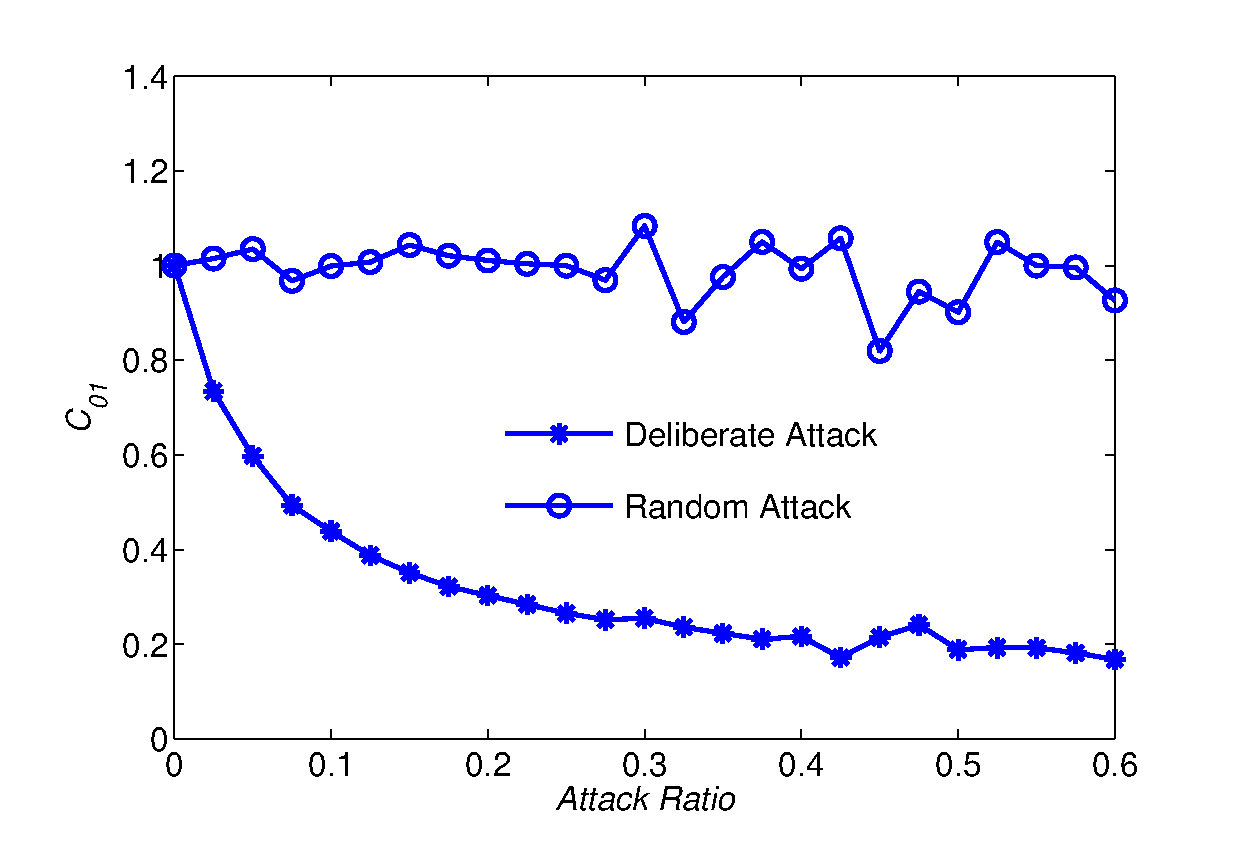
\epsfig{file=13a.eps, height=4cm, width=6cm}
\parbox{15.5cm}{\footnotesize \hspace{2.5cm}(a) HPN.}
\end{minipage}
\begin{minipage}{0.3\linewidth}
    \centering
 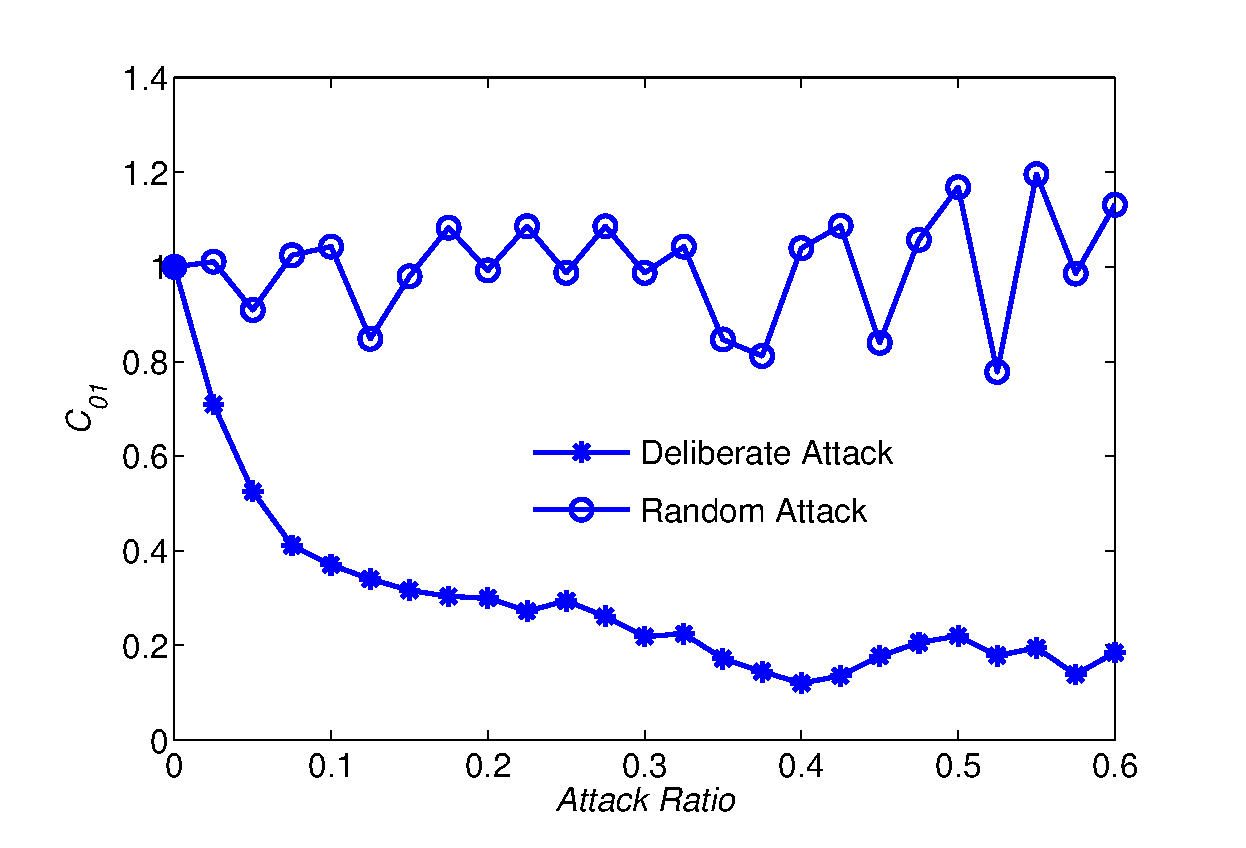
\epsfig{file=13b.eps, height=4cm, width=6cm}
 \parbox{15.5cm}{\footnotesize \hspace{2.3cm}(b) NHPN.}
\end{minipage}
\begin{minipage}{0.3\linewidth}
    \centering
 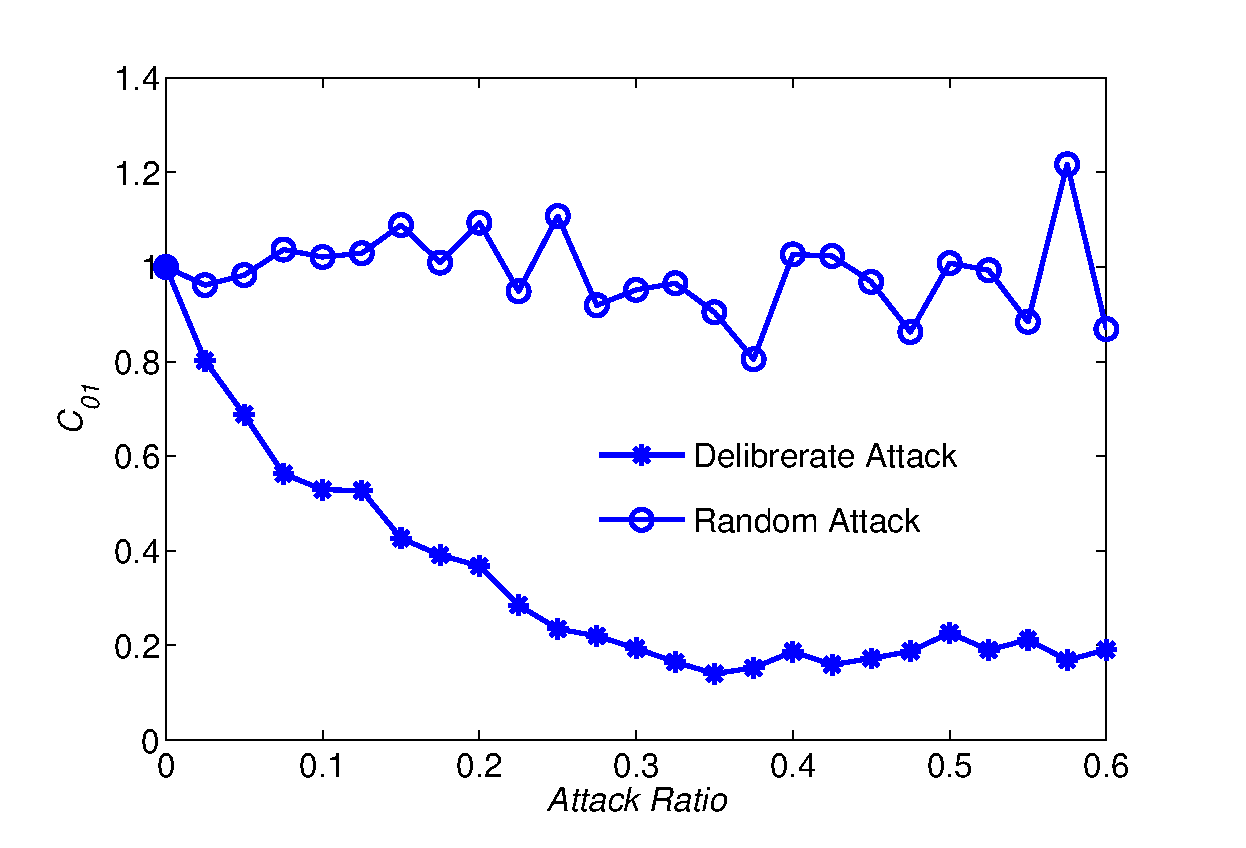
\epsfig{file=13c.eps, height=4cm, width=6cm}
 \parbox{15.5cm}{\footnotesize \hspace{2.5cm}(c) BDN.}
\end{minipage}
\hspace{3ex}
 \caption{\label{f9} Deliberate and random attack with different ratios to networks. Abscissa shows the ratio of attack and ordinate shows variation of average clustering  coefficient after the attack $C_{01}$.}
\end{figure*}
We also demonstrate the degree distributions and exponents in
double logarithmic in Fig. \ref{f9}, \ref{f10} and \ref{f11}. For
clarity, we only choose three values for each situation using
different colors blue, red, green, which means three different
degree distributions and exponents are shown in different colors
in each figure. The circles denote the vertices of empirical data,
$x$ axis indicates its degree $k$, and $y$ axis indicates its
corresponding probability or frequency, while the lines denotes
the fitted value, the slopes are the desired degree exponents (the
line is translated for clarity and the slope remains constant).

Three figures show the same trend, even with different $\lambda$
(Fig. \ref{f9}, \ref{f10}, \ref{f11} (a)), $\mu$ (Fig. \ref{f9},
\ref{f10}, \ref{f11} (b)) and $t$ (Fig. \ref{f9}, \ref{f10},
\ref{f11} (c)), indicating that they are all typical scale-free
networks. However, due to the rarefaction method we use, with the
same argument, the nonhomogeneous network possesses less vertices,
therefore, Fig. \ref{f9} shows fewer points than other two
figures. And for the same type of network, under the condition of
same $\mu$, different $\lambda$ and $t$, respectively, display the
approximate result since both two arguments increase total number
of vertices of networks, see Fig. \ref{f9}, \ref{f10}, \ref{f11}
(a) (c). In addition, under the condition of same $\lambda$ and
$t$, higher $\mu$ makes the points wider, the reason is that $\mu$
determines the number of connections, the high value will increase
the degree of vertex, and enlarge the distance of different
degrees $k$, which makes the plot fatter, see Fig. \ref{f9},
\ref{f10}, \ref{f11} (b).


In brief, getting rid of the noise in the beginnings and tails of
empirical distributions, all three types of networks display a
good Power-law character and follow our theoretical analysis.


\subsection{Reliability of Networks }
Complex network reliability indicates the ability of a complex
network to perform its original function even when damaged by
natural or man-made attacks. Evaluations for reliability are
invulnerability and survivability, generally, measured by average
path length and clustering coefficient.


The first argument is the average path length, the reason for
choosing it is that it can perform the connectivity of network. In
general, the lower the average search step, the better the
connectivity. Therefore, comparing the network before and after
the attack, we can learn the strength and hazard of the attack
\cite{feng}. Suppose $l_{0}$ denotes the average path length of
the original network, $l_{1}$ denotes the average path length
after the first attack, then
\begin{equation}\label{e49}\footnotesize
L_{01}=\frac{l_{1}}{l_{0}},
\end{equation}
where $L_{01}$ denotes the strength and hazard of the first
attack. If the network is immune to any attack, then
$L_{01}$$=$$1$, the network is steady and unbreakable; if
$L_{01}$$<$$1$ after the first attack, if the connectivity
improves and, moreover, $L_{01}$ deviates further than $1$, this
implies the network's connectivity has become stronger, and the
network becomes more reliable; and if $L_{01}$$>$$1$ after the
first attack, if the connectivity gets worse and, moreover,
$L_{01}$ deviates further than $1$, this implies the network's
connectivity has become weaker, and the network becomes more
unreliable.

Similarly, another argument for measuring reliability is the
clustering coefficient. As we know, the clustering coefficient of
one vertex indicates its local connectivity, so the average
clustering coefficient can denote the connectivity of the whole
network. Suppose $c_{0}$ denotes the average clustering
coefficient of the original network, $c_{1}$ denotes the average
clustering coefficient after the first attack, then
\begin{equation}\label{e50}\footnotesize
C_{01}=\frac{c_{1}}{c_{0}},
\end{equation}
where $C_{01}$ denotes the strength and hazard of the first
attack. The principle of $C_{01}$ is same as $L_{01}$.


%If the network is immune to any attack, then $C_{01}$$=$$1$, the
%network is steady and unbreakable; if $C_{01}$$<$$1$ after the
%first attack, if the connectivity improves and, moreover, $C_{01}$
%deviates further than $1$, this implies the network's connectivity
%has become stronger, and the network becomes more reliable; and if
%$C_{01}$$>$$1$ after the first attack, if the connectivity gets
%worse and, moreover, $C_{01}$ deviates further than $1$, this
%implies the network's connectivity has become weaker, and the
%network becomes more unreliable.

The other issue is the attack itself. Generally, there are two
kinds of attacks: deliberate and random attack. The deliberate
attack operate with certain strategies to remove vertices and
edges, and usually caused by human factors. Contrarily, the random
attack remove vertices and edges with no purpose, and always
caused by self factors. %The reliability of networks can be divided
%into the anti-attack ability and fault tolerance, which correspond
%to deliberate and random attack, respectively. In this experiment,
%we remove certain percentages of highest degree vertices to
%simulate the deliberate attack, and remove certain percentages of
%random vertices to simulate the random attack.


The first experiment runs in the same scale of three kinds of
networks. The execution time of all networks is $500$, For HPN,
the input rate $\lambda$$=$$4$, for NHPN, the input rate $\lambda
(t)$$ \leq$$\lambda =4$ which follows Eq. \ref{e32}, and for BDN,
the input rate $\lambda$$=$$4$ and output rate $\nu$$ =$$1$. For
each network, we record its original average path length and
clustering coefficient as $l_{0}$ and $c_{0}$, then, attack
networks deliberately and randomly and record the length and
coefficient after attack as $l_{1}$ and $c_{1}$. Eq. \ref{e49} and
\ref{e50} are employed to calculate the changing rate, the results
of deliberate and random attack are displayed in Fig. \ref{f8} and
\ref{f9}, respectively. From these two figures, we can obviously
see the different results. All three kinds of networks display
great vulnerability to deliberate attack, the change of average
path length increases intensively with the growth of attack ratio
while average clustering coefficient drops rapidly, the underlying
reason is the inhomogeneity of degree distribution, the less
vertices occupy the most degree, once they were removed from
network, most connections are cut off, and shortcuts are also
destroyed and gathering degree decreases, on the diagram, it
displays the $L_{01}$ grows, see Fig. \ref{f8} (a), (b) and (c),
plots with circular markers, and $C_{01}$ drops, see Fig. \ref{f9}
(a), (b) and (c), plots with circular markers. Unlike the
deliberate attack, all three networks display strong robustness to
random attack, both the average path length and clustering
coefficient keeps steady, since the most vertices occupy the low
degree, which is less important in the whole network, and the
random attack mostly works on these low degree vertices,
therefore, the connectivity and clustering of the whole network
hardly change, on the diagram, it displays $L_{01}$ and $C_{01}$
keeps a straight line, see Fig. \ref{f8} and \ref{f9} (a), (b) and
(c), plots with star markers.

%listed in Tab. \ref{t5} in the appendix (HPN: $l_{0}$$=$$2.5088$,
%$c_{0}$$=$$0.1087$, NHPN: $l_{0}$$=$$2.2290$, $c_{0}$$=$$0.1267$,
%BDN: $l_{0}$$=$$2.2220$, $c_{0}$$=$$0.1088$) and \ref{t6} (HPN:
%$l_{0}$$=$$2.5088$, $c_{0}$$=$$0.1087$, NHPN: $l_{0}$$=$$2.2290$,
%$c_{0}$$=$$0.1267$, BDN: $l_{0}$$=$$2.2220$, $c_{0}$$=$$0.1088$).
%The attack ratio shows the level of attack and is denoted as
%$\frac{m}{n}$, $n$ is the number of vertices in the whole network
%while $m$ is the number of the removed vertices. Obviously, to all
%three kinds of networks, with the increase of attack ratio, the
%deliberate attack significantly influent the connectivity, the
%average path length increases rapidly, and the average clustering
%coefficient drops rapidly, which both lead to decrease of
%connectivity, in contrast, the random attack has a slight
%influence, both the average path length and clustering coefficient
%are stable.



%For example, when the ratio of the deliberate attack is $0.05$,
%and the scale of network is $2000$, that means, we remove the
%$100$ highest degree vertices.




\begin{figure*}[t!]
\centering
\begin{minipage}[b]{0.3\linewidth}
\centering
 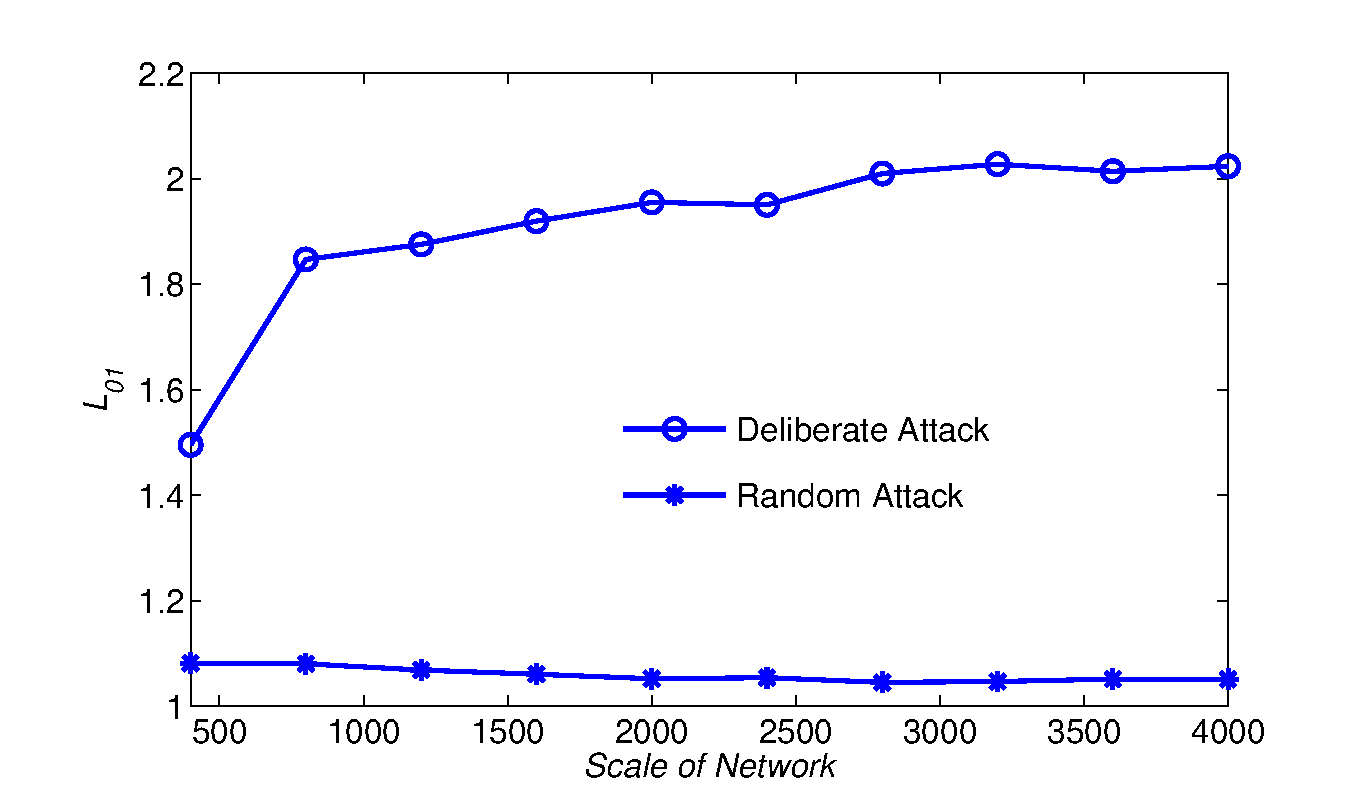
\epsfig{file=14a.eps, height=4cm, width=6cm}
\parbox{15.5cm}{\footnotesize \hspace{2.5cm}(a) HPN.}
\end{minipage}
\begin{minipage}[b]{0.3\linewidth}
    \centering
 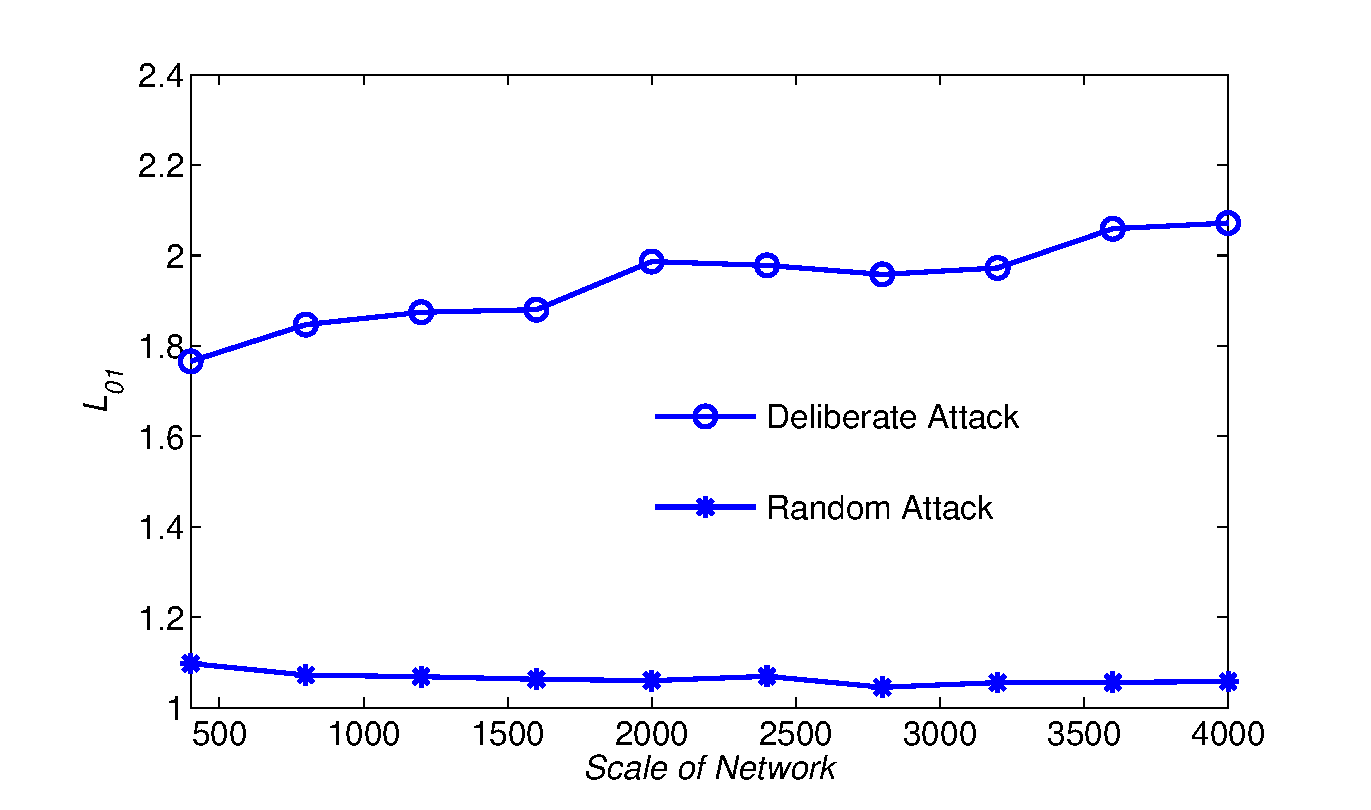
\epsfig{file=14b.eps, height=4cm, width=6cm}
 \parbox{15.5cm}{\footnotesize \hspace{2.3cm}(b) NHPN.}
\end{minipage}
\begin{minipage}[b]{0.3\linewidth}
    \centering
 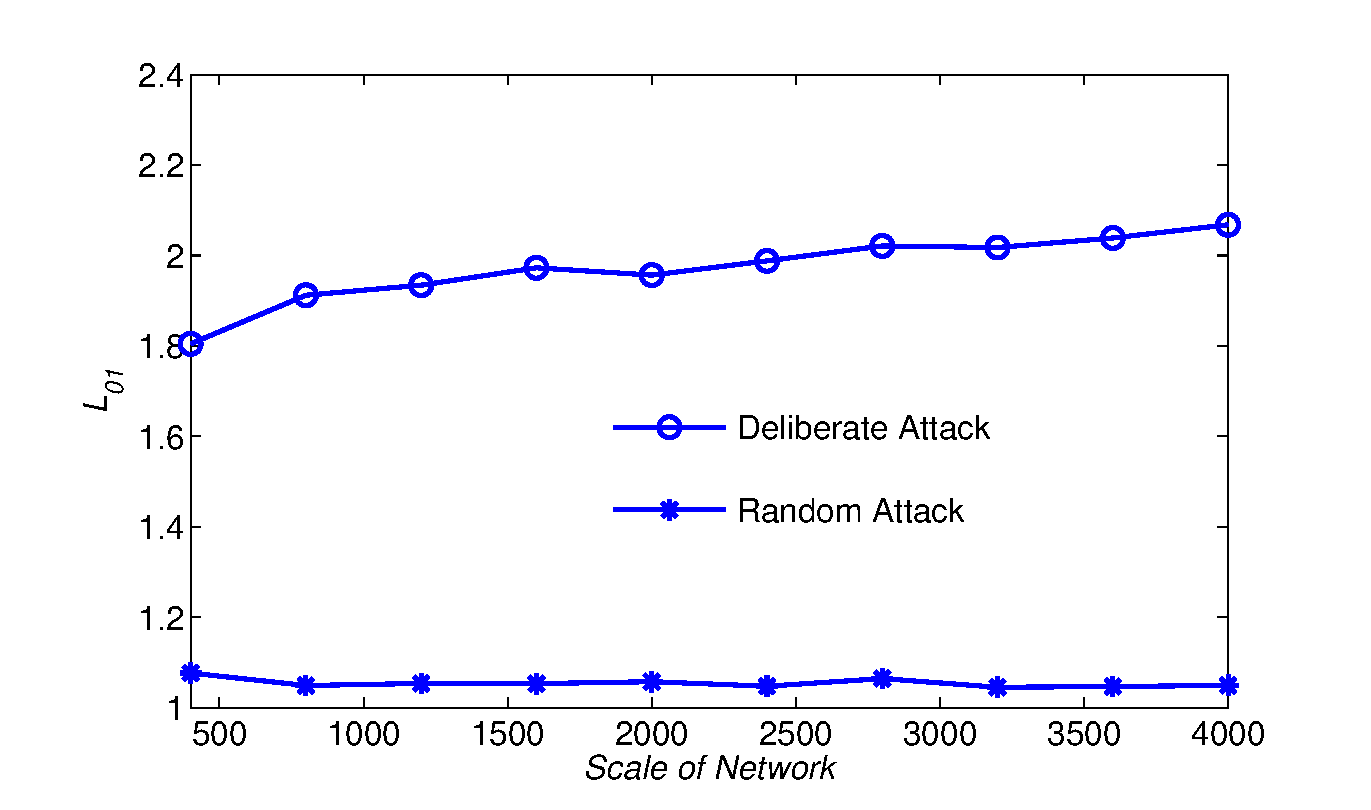
\epsfig{file=14c.eps, height=4cm, width=6cm}
 \parbox{15.5cm}{\footnotesize \hspace{2.5cm}(c) BDN.}
\end{minipage}
\hspace{3ex}
 \caption{\label{f10} Deliberate and random attack to networks with different scales. Abscissa shows the scale of network and ordinate shows variation of average path length after the attack $L_{01}$.}
\end{figure*}
\begin{figure*}
\centering
\begin{minipage}{0.3\linewidth}
\centering
 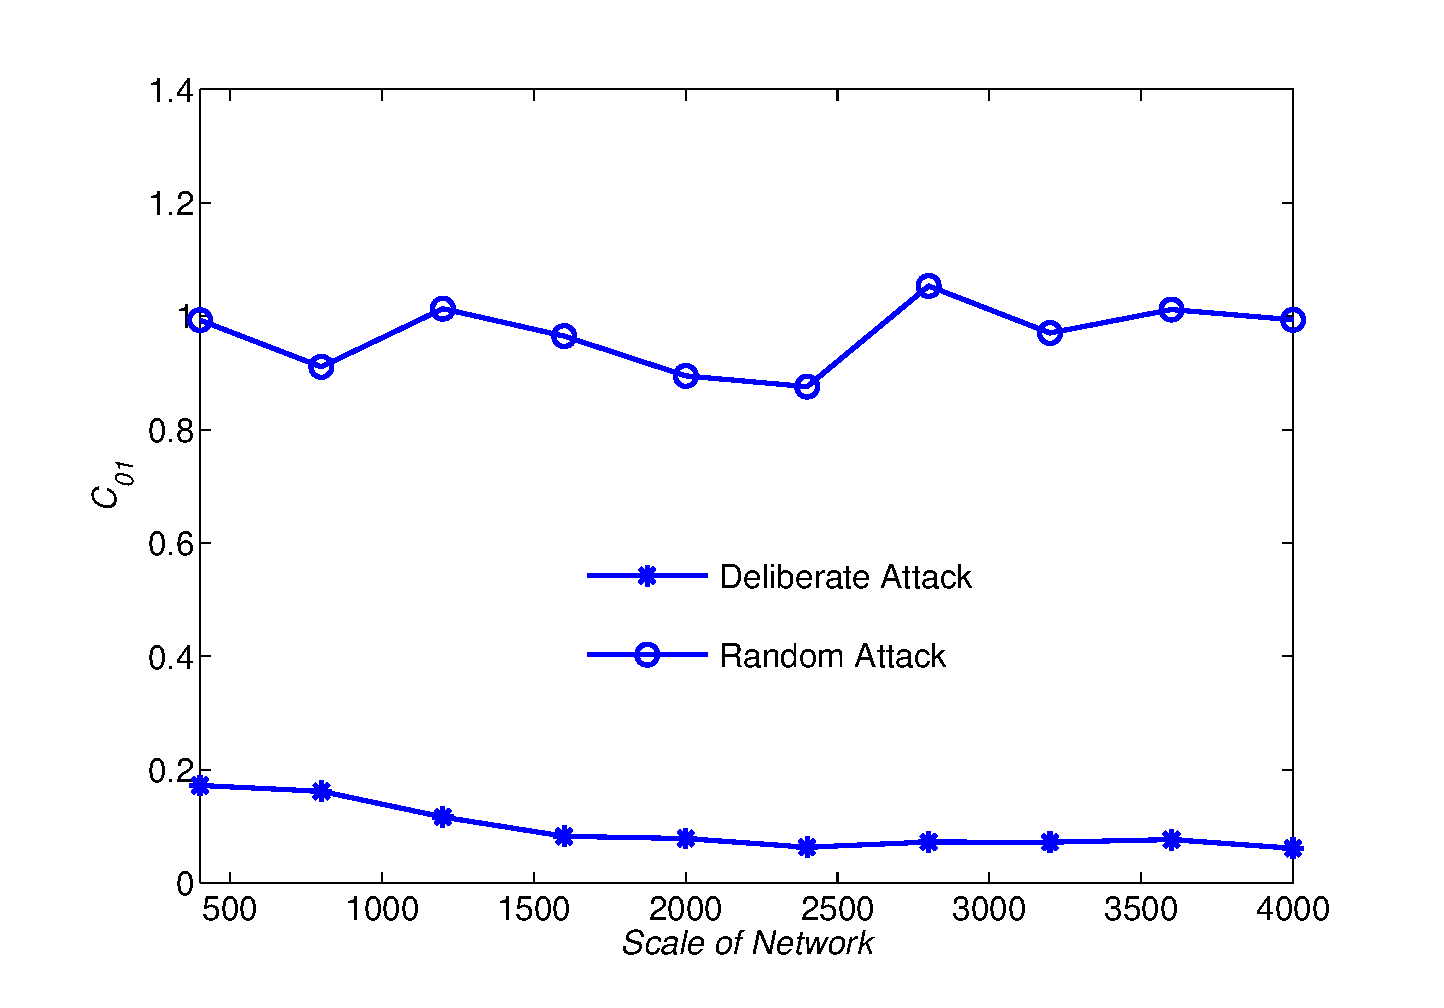
\epsfig{file=15a.eps, height=4cm, width=6cm}
\parbox{15.5cm}{\footnotesize \hspace{2.5cm}(a) HPN.}
\end{minipage}
\begin{minipage}{0.3\linewidth}
    \centering
 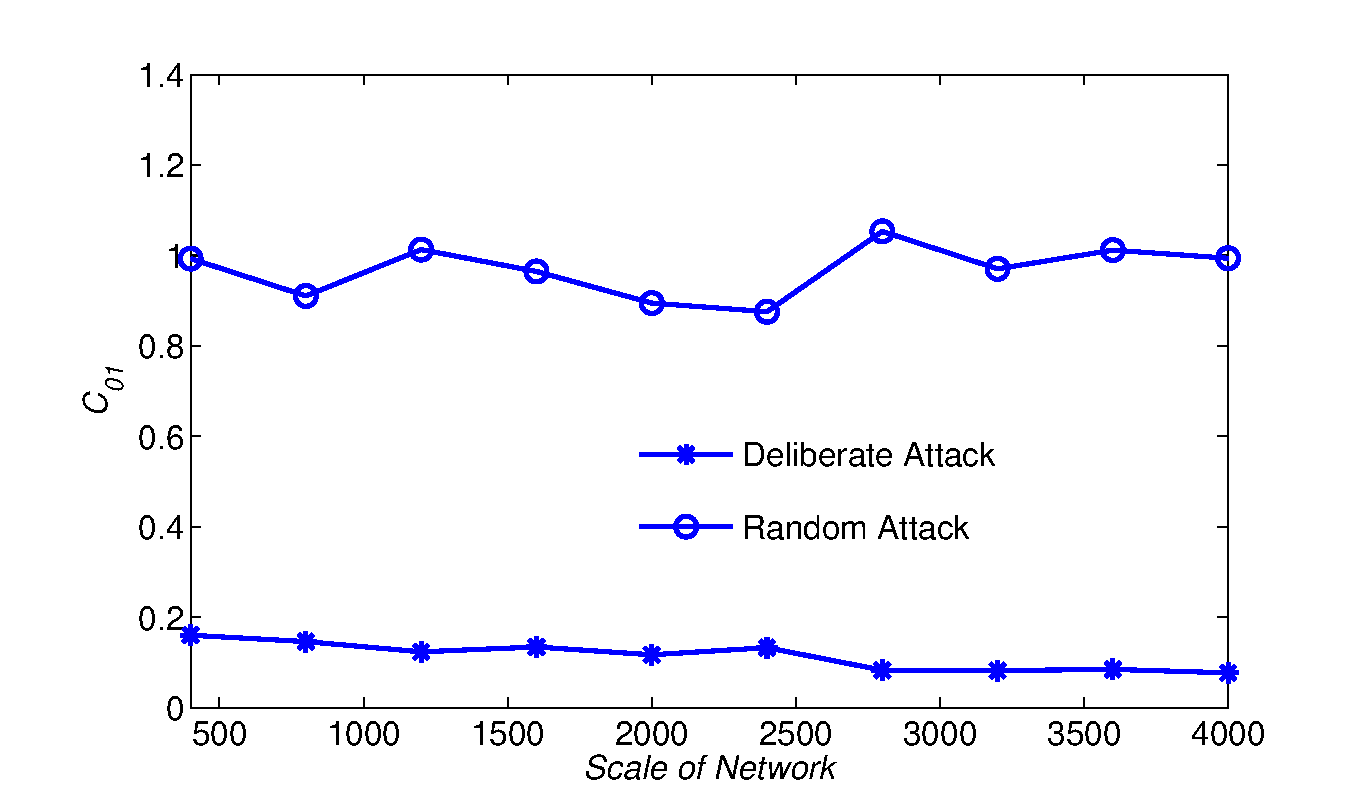
\epsfig{file=15b.eps, height=4cm, width=6cm}
 \parbox{15.5cm}{\footnotesize \hspace{2.3cm}(b) NHPN.}
\end{minipage}
\begin{minipage}{0.3\linewidth}
    \centering
 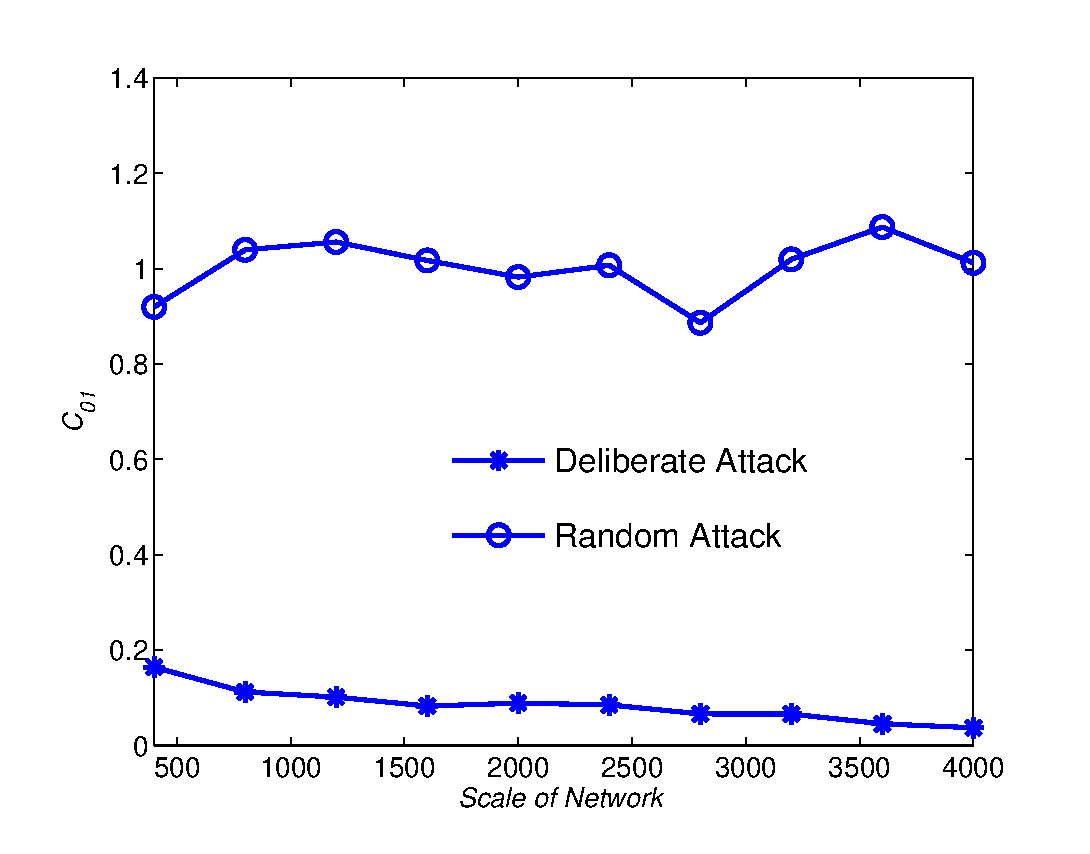
\epsfig{file=15c.eps, height=4cm, width=6cm}
 \parbox{15.5cm}{\footnotesize \hspace{2.5cm}(c) BDN.}
\end{minipage}
\hspace{3ex}
 \caption{\label{f11} Deliberate and random attack to networks with different scales. Abscissa shows the scale of network and ordinate shows variation of average clustering  coefficient after the attack $C_{01}$.}
\end{figure*}



%\begin{table}[t!]\tiny
%\begin{center}
%\caption{\label{t5} Deliberate attack to three kinds of networks}.
%\begin{tabular}{|c|cc|cc|cc|}
% \hline
%   Attack  &\multicolumn{2}{c|}{HPN} &\multicolumn{2}{c|}{NHPN}&\multicolumn{2}{c|}{BDN}\\
%   \cline{2-7} Ratio &$l_{1}$ &$c_{1}$ &$l_{1}$ &$c_{1}$  &$l_{1}$ &$c_{1}$ \\
%  \hline
%   0.05    &2.7903 &0.0649 &2.4561 &0.0666 &2.3783 &0.0748\\
%  \hline
%   0.10    &3.0277 &0.0476 &2.6124 &0.0469& 2.5137 &0.0575\\
% \hline
%   0.15    &3.2711 &0.0382 &2.7540 &0.0401 & 2.6283 &0.0464\\
% \hline
%   0.20    &3.5069 &0.0329 &2.9318 &0.0381 & 2.7809 &0.0400\\
%    \hline
%   0.25    &3.7770  &0.0288 &3.1122 &0.0373 & 2.9601 &0.0255\\
%    \hline
%   0.30    &4.0656 &0.0277 &3.3626 &0.0277 & 3.2970 & 0.0211\\
%   \hline
%     0.35    &4.3943 &0.0242 &3.6922 &0.0218 &3.4112 &0.0153\\
%  \hline
%   0.40    &4.8793 &0.0235 &4.0960 &0.0152 & 3.8338 &0.0203\\
% \hline
%   0.45    &5.5545 &0.0233 &4.5705 &0.0225 & 4.4365 & 0.0204\\
% \hline
%   0.50    &6.1725 &0.0205 &4.8371 &0.0279 & 5.0206 &0.0247\\
%    \hline
%   0.55    &7.2802 &0.0209 &5.7972 &0.0247 &5.9194 &0.0231\\
%    \hline
%   0.60    &6.1725 &0.0182 &7.3835 &0.0235 & 6.5694 & 0.0208\\
%   \hline
%\end{tabular}
%\end{center}
%\begin{center}\tiny
%\caption{\label{t6} Random attack to three kinds of networks}.
%\begin{tabular}{|c|cc|cc|cc|}
% \hline
%   Attack &\multicolumn{2}{c|}{HPN} &\multicolumn{2}{c|}{NHPN}&\multicolumn{2}{c|}{BDN}\\
%    \cline{2-7} Ratio &$l_{1}$ &$c_{1}$ &$l_{1}$ &$c_{1}$  &$l_{1}$ &$c_{1}$ \\
%  \hline
%   0.05    &2.5550 &0.1125 &2.2619 &0.1152& 2.2375 &0.1068\\
%  \hline
%   0.10    &2.5293 &0.1086 &2.2427 &0.1322 &2.2289 &0.1110\\
% \hline
%   0.15    &2.5309 &0.1134 &2.2744 &0.1242 & 2.2482 &0.1183\\
% \hline
%   0.20    &2.5698 &0.1098 &2.3134 &0.1217 & 2.2576 &0.1189\\
%    \hline
%   0.25    &2.5679 &0.1087 &2.3181 &0.1258 & 2.2495 &0.1204\\
%    \hline
%   0.30    &2.6057 &0.1178 &2.3329 &0.1251 & 2.3653 &0.1034\\
%   \hline
%     0.35    &2.7174 &0.1061 &2.4022 &0.1073 & 2.4170 &0.0983\\
%  \hline
%   0.40    &2.7095 &0.1080 &2.2848 &0.1317 & 2.3878 &0.1116\\
% \hline
%   0.45    &2.6365 &0.0891 &2.4579 &0.1064 & 2.3535 &0.1053\\
% \hline
%   0.50    &2.6937 &0.0980 &2.3144 &0.14805 & 2.3963 &0.1096\\
%    \hline
%   0.55    &2.7366 &0.1087 &2.3412 &0.1516 &2.3519 &0.0961\\
%    \hline
%   0.60    &2.7719 &0.1007 &2.3884 &0.1434 & 2.4851 &0.0945\\
%   \hline
%\end{tabular}
%\end{center}
%\end{table}
%
%
%
%
%
%
%\begin{table}[t!]\tiny
%\begin{center}
%\caption{\label{t7} The arguments of original networks}.
%\begin{tabular}{|c|cc|cc|cc|}
% \hline
% Network  &\multicolumn{2}{c|}{HPN} &\multicolumn{2}{c|}{NHPN}&\multicolumn{2}{c|}{BDN}\\
%   \cline{2-7} Scale &$l_{0}$ &$c_{0}$ &$l_{0}$ &$c_{0}$  &$l_{0}$ &$c_{0}$ \\
%  \hline
%  400    &2.1071 &0.1160 &2.1025 &0.1209 &2.1661 &0.0980 \\
%  \hline
%   800    &2.1903 &0.0981 &2.3275 &0.0687 & 2.3759 &0.0631\\
% \hline
%   1200    &2.4207 &0.0557 &2.4016 &0.0601 & 2.5087 &0.0446 \\
% \hline
%   1600    &2.4940 &0.0466&2.5042 &0.0456 & 2.5670 &0.0395  \\
%    \hline
%   2000    &2.5573  &0.0392 &2.5558 &0.0400 & 2.6117 &0.0344\\
%    \hline
%   2400    &2.6071 &0.0337 &2.5951 &0.0371 & 2.6746 & 0.0275\\
%   \hline
%   2800    &2.6372 &0.0314 &2.6320 &0.0330 &2.6987 &0.0258 \\
%  \hline
%   3200    &2.6677 &0.0287 &2.6753 &0.0271 & 2.7238 &0.0232 \\
% \hline
%   3600    &2.6850 &0.0271 &2.6945 &0.0261 & 2.7479 & 0.0216\\
% \hline
%   4000    &2.7085 &0.0249 &2.7104 &0.0248 & 2.7614 &0.0206 \\
%   \hline
%\end{tabular}
%\end{center}
%\begin{center}
%\caption{\label{t8} The arguments of networks after deliberate
%attack}.
%\begin{tabular}{|c|cc|cc|cc|}
% \hline
%    Network &\multicolumn{2}{c|}{HPN} &\multicolumn{2}{c|}{NHPN}&\multicolumn{2}{c|}{BDN}\\
%    \cline{2-7}Scale &$l_{1}$ &$c_{1}$ &$l_{1}$ &$c_{1}$  &$l_{1}$ &$c_{1}$ \\
%  \hline
%  400    &3.1511&0.0194 &3.7121 &0.0194 & 3.9087 &0.0161\\
%  \hline
%   800     &4.2485 &0.0118 &4.2989 &0.0101 &4.5428 &0.0071\\
% \hline
%   1200    &4.5394 &0.0065 &4.5013 &0.0074 &4.8527 &0.0045\\
% \hline
%   1600    &4.7873 &0.0038 &4.7092 &0.0061 &5.0633 &0.0033\\
%    \hline
%   2000    &4.9994 &0.0031 &5.0772 &0.0047 &5.1099 &0.0030\\
%    \hline
%   2400    &5.0846 &0.0021 &5.1330 &0.0049 & 5.3173 &0.0023\\
%   \hline
%   2800    &5.2996 &0.0022 &5.1535  &0.0027 & 5.4537 &0.0017\\
%  \hline
%   3200    &5.4089 &0.0021 &5.2761 &0.0022 & 5.4956 &0.0015\\
% \hline
%   3600    &5.4071 &0.0021 &5.5474 &0.0022 & 5.6022 &0.0010\\
% \hline
%   4000    &5.4804 &0.0015 &5.6149 &0.0019 & 5.7095 &0.0008\\
%    \hline
%\end{tabular}
%\end{center}
%\begin{center}
%\caption{\label{t9} The arguments of networks after random
%attack}.
%\begin{tabular}{|c|cc|cc|cc|}
% \hline
%    Network &\multicolumn{2}{c|}{HPN} &\multicolumn{2}{c|}{NHPN}&\multicolumn{2}{c|}{BDN}\\
%    \cline{2-7} Scale&$l_{1}$ &$c_{1}$ &$l_{1}$ &$c_{1}$  &$l_{1}$ &$c_{1}$ \\
%  \hline
%  400    & 2.2784 &0.10797 &2.3078 &0.1200 &2.3319 &0.0901\\
%  \hline
%   800    &2.4854 &0.0658 &2.4947 &0.0626 &2.4926 &0.0655\\
% \hline
%   1200    &2.5865 &0.0525 &2.5666 &0.0609 & 2.6428 &0.0471\\
% \hline
%   1600    &2.6455 &0.0450 &2.6609 &0.0440 & 2.7037 &0.0402\\
%    \hline
%   2000    &2.6909 &0.0386 &2.7087 &0.0358 & 2.7619 &0.0338\\
%    \hline
%   2400    &2.7481 &0.0343 &2.7745 &0.0325 & 2.8014 &0.0277\\
%   \hline
%   2800    &2.7565 &0.0348 &2.7512 &0.0348 & 2.8665 &0.0235\\
%  \hline
%   3200    &2.7932 &0.0308 &2.8234 &0.0263 & 2.8467 &0.0136\\
% \hline
%   3600    &2.8161 &0.0274 &2.8451 &0.0265 & 2.8760 &0.0235\\
% \hline
%   4000    &2.8475 &0.0242 &2.8667 &0.0247 & 2.8973 &0.0209\\
%    \hline
%\end{tabular}
%\end{center}
%\end{table}




The other experiment focuses on the relationship between
relationship between reliability and scale of the network. The
argument setting is as follows: for HPN, the input rate $\lambda$
$=$$4$, for NHPN, the input rate $\lambda (t)$$ \leq $$\lambda$$
=4$ which follows Eq. \ref{e32}, and for BDN, the input rate
$\lambda $ =$4$ and output rate $\nu$$=$$1$, and we choose the
scale of network as $400$, $800$, $1200$, $1600$, $2000$, $2400$,
$2800$, $3200$, $3600$ and $4000$. For each network, we record its
original average path length and clustering coefficient as $l_{0}$
and $c_{0}$, then, attack networks deliberately and randomly,
record the length and coefficient after attack as $l_{1}$ and
$c_{1}$. The attack ratio is $0.5$ which means half of vertices
are removed. For clarity, plots of $L_{01}$ and $C_{01}$ are
displayed in Fig. \ref{f10} and \ref{f11}, respectively. From
these figures, we can see that the larger the networks are, the
less stable they are, that is to say, all three networks are
unreliable to deliberate attack, and immune to random when the
scale is large. The reason is that, in the constructing processes
of all three networks, the more vertices added to network means
that the degree of highest degree vertices will increase
continuously. Deliberate attack first aims at these high degree
vertices, once they are removed from the network, the distance of
their neighbors will potentially increase, see Fig. \ref{f10} (a),
(b) and (c), plots with circular markers, and the clustering will
decrease, see Fig. \ref{f11} (a), (b) and (c), plots with circular
markers, therefore, the large network shows vulnerability to
deliberate attack. However, with the increasing of network scale,
random attack has a very low probability to remove high degree
vertex, so the large network shows robustness to it, $L_{01}$,
$C_{01}$ stay around $1$, see Fig. \ref{f10}, \ref{f11} (a), (b)
and (c), plots with star markers.

% These tables obviously show that, to all three kinds
%of networks, with the growth of network scale, the deliberate
%attack causes larger damage, that is, the connectivity and
%clustering both drop, on the other side, these networks all show
%strong stability, and the larger network seems to be more
%reliable.


Both two simulations show that three proposed network models are
``robust yet fragile", which is a basic and significant character
for complex systems and scale-free networks \cite{al} \cite{j1}.

\section{Conclusion and Outlook}
Network modeling and degree distribution, which are most
significant research domains for complex networks, demand greater
attention and further study. In this paper, we introduce three
novel network models, based on homogeneous Poisson, nonhomogeneous
Poisson and Birth and Death process, respectively. Additionally,
we analyze their degree distribution, and obtain degree exponents
by applying the dynamics method and probabilistic approach.
Conclusively, simulations of network construction, statistical
degree distribution and network reliability are carried out to
show that our models are typical scale-free networks.

Our study reveals that, regardless of the input rate and
connections of individuals, once the network constructing
mechanism, such as ``the richer are getting richer, and the poor
poorer", is decided, the topology such as the degree distribution
of complex networks remains unchanged. More practically, the war
or financial crisis will not change the scale-free character of
social or financial networks, which can be described as a
nonhomogeneous Poisson process for complex systems applied to most
of real networks. Further, the $\lambda$ and $t$ determine the
scale of network, while our proof indicates that the degree
exponent is free of these two arguments, that is to say, no matter
the larger scale or smaller scale (which can be considered as the
subgraph of the large) networks are, their degree distributions
are identical. In that sense, we can study the small or original
type of complex systems to reveal the topology of larger scale.
Additionally, our models with different input rates follow and
further confirm the definition of Complex Systems and Networks
proposed by Barab$\acute{a}$si \cite{bx}, ``independent of their
age, function, and scope, converge to similar architectures".


However, we have a dilemma in solving the degree exponent of birth
and death network, which is more close to practical complex
networks. Besides, the constructing mechanism is required to be
more concrete to simulate the reality. Since the network modeling
and degree distribution are the key issues for complex networks,
it is worth exploring for perfect solution to build fit models and
seek for their degree exponents. Further, our models have
potential to simulate those practical networks which is difficult
to obtain data, and how to fit our models to them is also an issue
we will try to address.

\begin{thebibliography}{1}
%\bibitem{Mil} S. Milgram, The small world problem. {\it Psychology
%Today}, vol. 1, no. 1, pp. 61-67, 1967.
\bibitem{Watts1} D.J. Watts, S.H. Strogatz, Collective dynamic of `small-world' networks, {\it Nature}, vol. 393, pp. 440-442, 1999.
\bibitem{Newman1} M.E.J. Newman, D.J. Watts, Renormalization group analysis of the small-world network model, {\it Physical Letter A}, vol. 263, no. 6, pp. 341-346, 1999.
\bibitem{Barabasi} A.L. Barab\'{a}si, R. Albert, Emergence of scaling in random networks, {\it Science}, vol. 286, pp. 509-512, 1999.
\bibitem{bah} A.L. Barab\'{a}si, R. Albert, H. Jeong, Mean-field
theory for scale-free random networks, {\it Physica A}, vol. 272,
no. 1-2, pp. 173-187, 1999.
\bibitem{kraa} P.L. Krapivsky, S. Render, F. Leyvraz, Connectivity
of growing random networks. {\it Physical Review Letter}, 85:
4629, 2000.
\bibitem{do} S.N. Dorogovtsev, J.F.F. Mendes, A.N. Samukhin,
Structure of growth networks with preferential linking, {\it
Physical Review Letter}, 85: 4633, 2000.
\bibitem{doro} S.N. Dorogovtsev, J.F.F. Mendes, Effect of the accelerating growth of communication networks on their structure, {\it Physical Review E}, 63: 025101, 2001.
\bibitem{jeong} H. Jeong, Z. NDA, A.L. Barab\'{a}si, Measuring preferential attachment in evolving networks, {\it Europhysics Letters}, vol. 61, pp. 567-572, 2003.
\bibitem{kra} P.L. Krapivsky, S. Redner, Network growth by coping, {\it Physical Review E}, 63: 036118, 2005.
\bibitem{li} X. Li, G.R Chen, A local world evolving network model, {\it Physica A}, vol. 328, pp. 274-286, 2003.
\bibitem{cs} C. Seshadhri, T.G. Kolda, A. Pinar, Community structure and scale-free collections of Erd\"{o}s-R\'{e}nyi
graphs, {\it Physical Review E}, 85: 056109, 2012.
\bibitem{houu} H. Su, M.Z.Q. Chen, J. Lam, Z. Lin, Semi-global leader-following consensus of linear multi-agent systems with input saturation via low gain
feedback, {\it IEEE Transacations on Circuits and Systems I:
Regular Papers}, vol. 60, no. 7, pp. 1881-1889, 2013.
\bibitem{guang} G. Wen, W, Yu, M.Z.Q. Chen, X. Yu, G. Chen, ${\cal H}_{infty}$ pinning synchronization of directed networks with aperiodic sampled-data communications, {\it IEEE Transacation on Circuits and Systems I: Regular Papers}, vol. 61, no. 11, pp. 3245-3255, 2014.
\bibitem{lian} W. Lian, R.G. Dromey, D. Kirk, Software engineering and scale-Free
Networks, {\it  IEEE Transactions on Systems, Man, and
Cybernetics, Part B: Cybernetics}, vol. 39, no. 3, pp. 648-657,
2009.
\bibitem{wen} W. Yu, J. Cao, G. Chen, J. Lu, J. Han, W. Wei, Local synchronization of a complex network
model, {\it  IEEE Transactions on Systems, Man, and Cybernetics,
Part B: Cybernetics}, vol. 39, no. 1, pp. 230-241, 2009.
\bibitem{span} M.C. Spencer, J.H. Downes, D. Xydas, M.W. Hammond, V.M. Becerra, K. Warwick, B.J. Whalley, S.J.
Nasuto, Multiscale evolving complex network model of functional
connectivity in neuronal cultures, {\it IEEE Transactions on
Biomedical Engineering}, vol. 59, no. 1, pp. 30-34, 2012.
\bibitem{hou} H. Su, Z. R, M.Z.Q. Chen, X. Wang, G. Chen, H. Wang,
Decentralized adaptive pinning control for cluster synchronization
of complex dynamical networks, {\it IEEE Transactions on
Cybernetics}, vol. 43, no. 1, pp. 394-399, 2013.
\bibitem{sc} M.N. Schmidt, M. Morup, Nonparametric bayesian modeling of complex networks: an
introduction, {\it IEEE Signal Processing Magazine}, vol. 30, no.
3, pp. 110-128, 2013.
\bibitem{ma} N. Mahdavi, M.B. Menhaj, J. Kurths, J. Lu, Fuzzy complex dynamical networks and its
synchronization, {\it IEEE Transactions on Cybernetics}, vol. 43,
no. 2, pp. 2168-2267, 2013.
\bibitem{data} M. E. J. Newman, Finding community structure in networks using the eigenvectors of
matrices, {\it Physical Review E}, 74: 036104, 2006.
\bibitem{jeong1} H. Jeong, B. Tombor, R. Albert, Z. N. Oltvai, A.-L.
Barab\'{a}si, The large-scale organization of metabolic networks,
{\it Nature}, vol. 407, pp. 651-654, 2000.
\bibitem{sta} S. Milojevi\'{c}, Power-law distributions in information science: Making the case for logarithmic
binning, {\it Journal of the American Society for Information
Science and Technology}, vol. 61, no. 12, pp. 2417-2425, 2010.
\bibitem{h} H. Bauke, Parameter estimation for power-law distributions by maximum likelihood
methods, {\it The European Physical Journal B}, vol. 58, no. 2,
pp. 167-173, 2007.
\bibitem{aa} A. Clauset, C. R. Shalizi, M. E. J. Newman, Power-law distributions in empirical data, {\it SIAM review}, vol. 51, no. 4, pp. 661-703, 2009.
\bibitem{vi} Y. Virkar, A. Claust, Power-law distributions in binned empirical
data, {\it The Annals of Applied Statistics}, vol. 8, no. 1, pp.
89-119, 2014.
\bibitem{feng} M. Feng, H. Qu, Y. Zhang, Highest degree likelihood search algorithm using a state transition matrix for complex
networks, {\it IEEE Transactions on Circuits and Systems I:
Regular Papers}, vol. 61, no. 10, pp. 2941-2950, 2014.
\bibitem{al} R. Albert, H. Jeong, A.L. Barab\'{a}si, Attack and error tolerance of complex networks, {\it Nature}, vol. 406, pp. 378-382, 2000.
\bibitem{j1} J.M. Carlson, J. Doyle, Highly optimized tolerance: Robustness and design in complex systems, {\it Physical Review Letters}, 84: 2529, 2000.
\bibitem{bx} A.L. Barab\'{a}si, Scale-free networks: a decade and beyond, {\it Science},
vol. 325, pp. 412-413, 2009.
\end{thebibliography}


\bibliographystyle{IEEETran}
\begin{biography}[{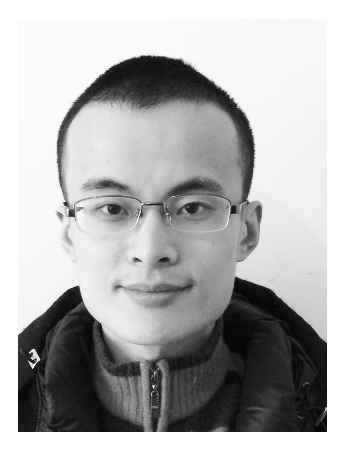
\includegraphics[width=1in,clip,keepaspectratio]{Feng_photo}}]{Minyu Feng}
is currently a Ph.D. student in University of Electronic Science
and Technology of China. He received the B.S. degree and the M.S.
degrees in computer science and engineering from the University of
Electronic Science and Technology of China, Chengdu, China, in
2010 and 2013, respectively. His research interests include
network topology, path seeking, social networks, optimization and
machine learning.
\end{biography}
\begin{biography}[{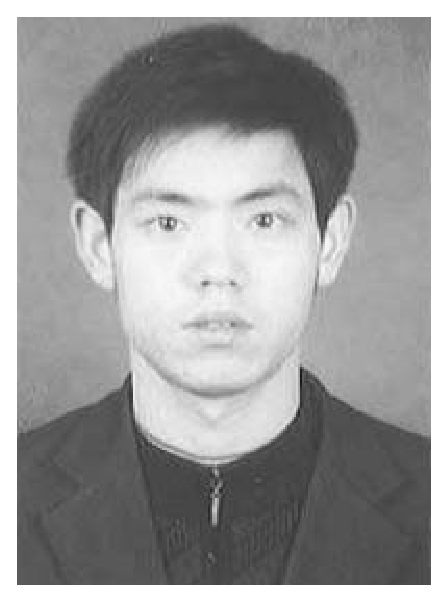
\includegraphics[width=1in,clip,keepaspectratio]{Qu_photo}}]{Hong Qu}
received the Ph.D. degree in computer science from the University of Electronic
Science and Technology of China, Chengdu, in 2006. Currently, he is a professor in the School of Computer Science and
Engineering, University of Electronic Science and Technology of
China. His current research interests include neural networks,
deep learning, intelligent computation, and optimization.
\end{biography}
\begin{biography}[{\includegraphics[width=1in,clip,keepaspectratio]{Yi_photo.eps}}]{Zhang Yi}
received the Ph.D. degree in mathematics from the
Institute of Mathematics, Chinese Academy of Science, Beijing,
China, in 1994. Currently, he is a Professor of College of Computer Science at Sichuan University.
His research interests include neural networks, big data, and machine learning.
\end{biography}
\begin{biography}[{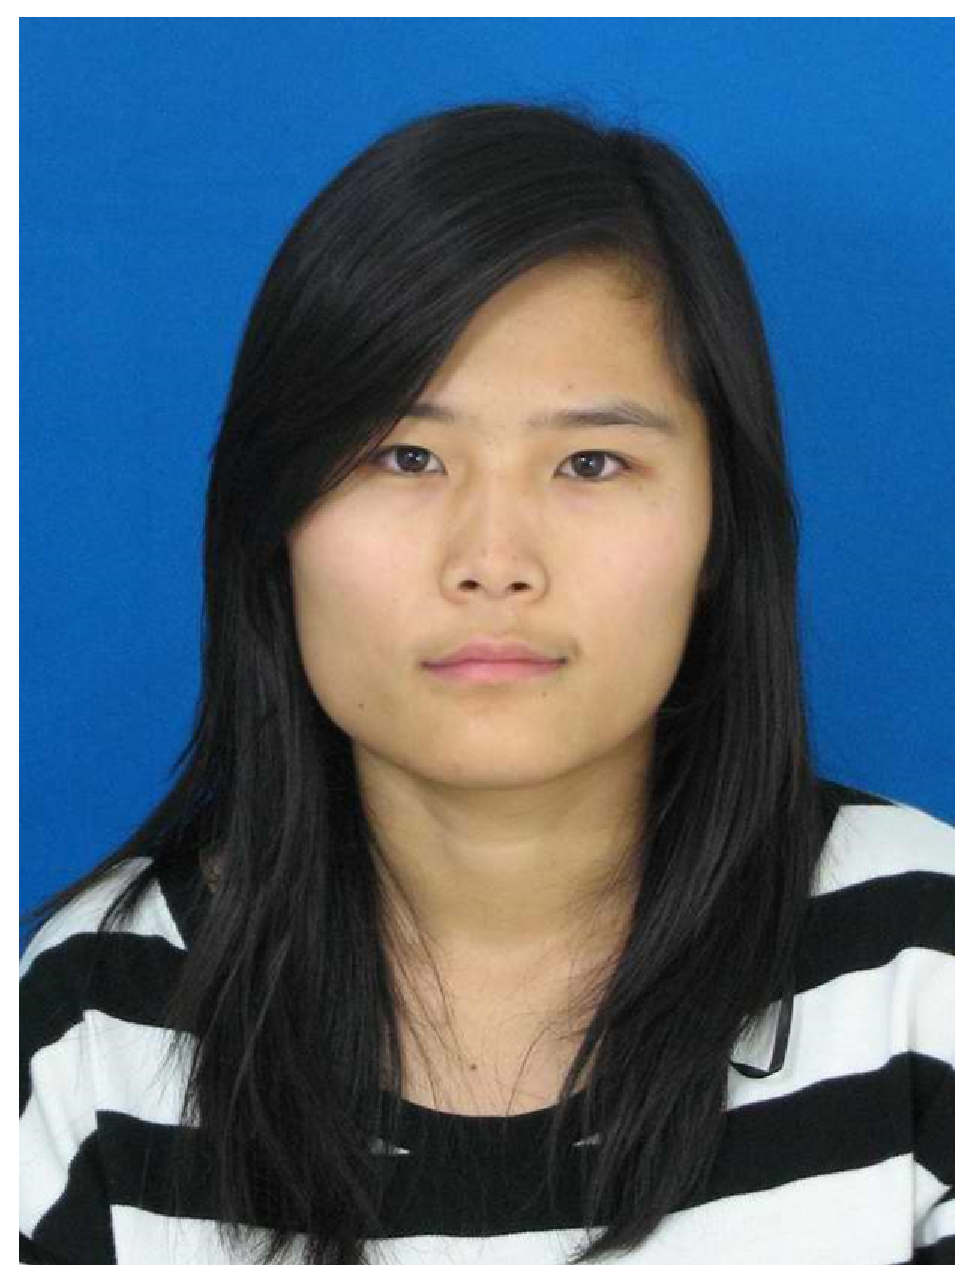
\includegraphics[width=1in,clip,keepaspectratio]{XiuruiXie.eps}}]{XiuruiXie}
 is a current Ph.D. student in Department of computer science and engineering, University of Electronic Science and Technology of China. Her current research interests relate to neural networks, intelligent computation, and optimization.
\end{biography}

\end{document}
